\input{thesis_default} % main tamplate

\begin{document}
%\input{title} % это титульный лист
%\input{diplom_task}
\tableofcontents % это оглавление, которое генерируется автоматически
\newpage

%\addcontentsline{toc}{chapter}{Введение}
\chapter*{Введение}

Большое количество современных систем являются беспроводными. Простота развертывания, мобильность, относительно низкая
стоимость, вот основные преимущества беспроводных систем. Количество мобильных устройств (телефоны, планшетные компьютеры
и т.д.) с каждым годом стремительно растет, только мобильных телефонов в 2011 году было 5.6 миллиарда и покрывало 79.86\%
\cite{wiki_mobilenum} населения земли. Технологии беспроводной связи глубоко проникли во все сферы жизни общества:
обеспечение безопасности с помощью RFID датчиков, предоставление доступа в интернет по технологиями 3G, Wi-Fi, 
сотовая связь по различным технологиям (GSM, CDMA, DAMPS). Некоторые из этих систем строятся на основе методики
расширения спектра, которая отвечает современным требованиям по мощности сигнала, а также по безопасности передаваемых
данных. В основе таких систем лежат шумоподобные (широкополосные) сигналы - ШПС. Вместе с тем растут требования к таким
системам. Применение ШПС ставит ряд специфических задач по обработке информации, обусловленных особенностями ШПС.
Свойства характерные для ШПС, выгодно отличают данный класс систем от класса узкополосных систем, но с другой стороны
оборачивается усложнением методов обработки ШПС.

Внедрение новых технологий требует увеличение полосы частот. Разнообразие технологий беспроводной передачи данных среди
гражданских и военных систем ведет к перегрузке каналов связи и все более высоким требованиям к скорости передачи
данных. С учётом данных требований применение систем передачи информации с ШПС становится все более востребованным.

Принимая во внимание географические размеры России и стратегическую важность обладания собственными системами спутникового
позиционирования, правительство Российский Федерации уделяет особое внимание разработке собственной системы
глобального спутникового позиционирования ГЛОНАСС. Обладание собственными технологиями системы спутниковой навигации (СНС), государство может обезопасить
себя в случае военных конфликтов от ограничения применения американской системы СНС Navstar GPS в зоне конфликта.

Разработка систем, позволяющих работать с несколькими различными СНС, позволит повысить точность определения координат
в сложных условиях города. Сложность детектирования сигнала и определения координат обусловлена наличием плотной
застройки многоэтажными зданиями. В городских условиях задача подавления интерференционной помехи становится особенно
актуальной. Спектр интерференционной помехи не является белым, а фильтрация и компенсация цветного шума
требует разработки специальных алгоритмов.

Новые цифровые процессоры позволяют применять подходы, которые еще 10-15 лет назад были бесперспективными.
В данной работе развиваются подходы на основе построения параметрической модели ШПС. Невозможность использования
методов требующих вычислений с высокой точностью в приемниках реального времени
10-15 лет назад была обусловлена слабой производительностью процессоров и микроконтроллеров, а также существенной
стоимостью процессоров с модулем для операций с числами с плавающей точкой. Современное развитие цифровых технологий делает 
возможным применение параметрических методов оценки спектра взамен традиционного подхода основанного на непараметрического
анализа спектра.

Основа теории систем связи с ШПС была заложена в работах В.А. Котельникова и К. Шеннона.
России в этой области занимаются В.И. Борисов, В.Б. Пестряков, В.И. Журавлев, М.И. Жодзишский, Б.И. Шахтарин, Л.Е.  Варакин, В.Е. Гантмахер и др.

Изначально методы расширенного спектра применялись при разработке военных систем управления и связи \cite{sklyar}.
К концу второй мировой войны расширение спектра применялось в радиолокации для борьбы с преднамеренными помехами, а
в последствии развитие данной технологии объяснялось желанием создать помехоустойчивые системы связи.
В конце 40-х-начале 50-х годов прошлого века Мортимер Рогофф, сотрудник Международной Телефонной и Телеграфной Корпорации (США) (ITT),
провёл эксперимент по передаче информации при помощи псевдошумового сигнала \cite{sklyar}, среди отечественных ученых
в середине 30-х годов прошлого века работу об основах кодового разделения каналов написал Д.В. Агеев.
Первые разработки таких систем относились к военным отраслям. Данный факт объясняется рядом особенностей, которыми обладают
сигналы с расширенным спектром, в числе которых — сложность перехвата заложенной в них информации,
высокая помехоустойчивость, а также трудность обнаружения факта работы передатчика. В процессе исследований расширенному спектру
нашлось и другое применение - снижение плотности энергии, высокоточная локация, использование при множественном доступе
\cite{sklyar}

Системы связи с широкополосными сигналами занимают особое место. Их особенные свойства выделяют данный класс из других систем
связи. Высокая помехозащищенность при действии сильной помехи, кодовое разделение большого количества абонентов, прием
информации с высокой достоверностью - отличительные особенности широкополосных система. Эти черты были известно, но
уровень элементной базы и низкий уровень помех не позволяли получить развития системам данного класса. Однако развитие
элементной привело к широкому распространению данного вида сигналов. В настоящее они применяются в системах спутниковой навигации,
системах сотовой связи и др \cite{varakin-book}.

Отношение сигнал/шум (ОСШ) на входе приемника может быть очень низким. Для обеспечения высокой помехозащищенности 
в таких случаях используются ШПС с большими и сверхбольшими базами.

К созданию сложных широкополосных сигналов (СШС) привело решение ряда проблем при развитии систем передачи данных.
Первая проблема встала при разработке новых радиолокационных система. Для дальнейшего развития требовалось
решить несколько противоречий: требование высокой разрешающей способности по дальности и дальностью обнаружения
целей в импульсных РЛС, требование точного измерения скорости и высокое разрешение по дальности, требование
увеличить дальность при ограничении пиковой мощности \cite{gantmaher-book}. Решение данных задач было предложено
Ф. Вудвардом. Им было показано, что дополнительным параметром является форма сигнала. Длительность сигнала
может быть больше - настолько больше, насколько это необходимо для обеспечения энергетических требований, а требование
разрешения по дальности и точности измерений определяются шириной полосы сигнала. Данные требования обеспечивается
путем сжатия импульса на стороне приемника. Вудворд сформулировал принципы: произведение эффективной полосы частот
радиосигнала на его длительность должен быть существенно больше единиц ${FT>>1}$, внутренняя структура сигнала
должна быть такой, чтобы обеспечить возможность приемнику сжатие распределенного во времени сигнала в короткий импульс,
соответствующий полосе ${F}$ \cite{gantmaher-book}.

В \cite{gantmaher-book} показана связь пропускной способности канала с понятием ШПС. При ${R_e<<1}$ можно записать:
\begin{equation}
	%\label{eq:shennon_cdma}
	FT = \frac{1}{\log(1+R_e)}, \nonumber
\end{equation}
где ${R_e}$ - ОСШ, ${F}$ - эффективная полоса частот, ${T}$ - длительность.

Стоить отметить, что при ${R_e<<1}$, левая часть данного выражения стремится к бесконечности, а значит
ШПС позволяет обеспечить теоретически неограниченную достоверность передачи информации. Второе важное свойство
ШПС - способность работать "под шумами". Что обеспечивает скрытность
передачи информации, а с другой высокую степень уплотнения каналов связи и, как следствие, решение современных проблем
с перегруженностью каналов связи.

В данной работе будет рассматриваться ШПС модулированный ПСП на основе двоичной рекуррентной последовательности.
Для выделения данных из потока необходимо иметь точно синхронизированную копию ПСП, которая была использована
при модулировании сигнала на передающей стороне. Для достижения синхронизма на стороне приемника необходимо
устранить неопределенность в двух областях: неопределенность по частоте и неопределенность по фазе (задержке) ПСП.
Неопределенность по фазе ПСП обусловлена неопределенностью в расстоянии между передатчиком и приемником. Неопределенность
по частоте обусловлена в первую очередь доплеровским эффектом, а также нестабильностью опорных генераторов в
передатчике и приемнике. После устранения неопределенности по частоте для достижения точной синхронизации
начинается процесс слежения за частотой. Неопределенность по фазе ПСП устранить, не используя полный перебор,
невозможно в силу корреляционных свойств ПСП. Таким образом можно заключить, что задача быстрого и эффективного
поиска и оценки параметров ШПС является актуальной.

В данной работе рассматривается подход программного приемника (Software Defined Receiver - SDR)
\cite{akos-book, grayver-book, pany-book} для оценки параметров ШПС. Как уже было отражено выше, ШПС применяется во
многих системах. В данной работе для полунатурного эксперимента будет рассматриваться сигнал СНС Navstar GPS. Данная система передачи 
информации (СПИ) использует ПСП Голда \cite{gold-ieee} для модулирования сигнала.

Традиционные подходы к реализации приемника СНС Navstar GPS отражены в \cite{akos-book, tsui}. 

Популярность и распространенность данной системы стимулирует исследования в области детектирования
и оценки параметров ШПС сигнала.

Существуют исследования в области применения теории хаоса - детектирование и оценка
частоты ШПС с применением осциллятора Дуффинга \cite{chaos_cambridge, chaos_chen, chaos_huang, chaos_wang}. Преимуществом
данного подхода является то, что свойства осциллятора позволяют детектировать сигналы с экстремально низким ОСШ.

Осциллятор Дуффинга с гармоническим внешним воздействием может быть описан уравнением:
\begin{equation}
	\label{eq:duffing}
	mx'' + cx' + k_{1}x + k_{2}x^3 = F_{0}\cos(\omega{t}),
\end{equation}
где $m$ - масса, $c$ - коэффициент диссипации, $x$ - состояние осциллятора, $k_1$ и $k_2$ - линейный и нелинейный коэффициенты соответственно,
$F_{0}\cos(\omega{t})$ - внешнее воздействие.

Подробно уравнение \ref{eq:duffing} рассмотрено в \cite{chaos_neimark_landa}.
Для использования осциллятора Дуффинга с целью оценки параметров ШПС была предложена усовершенствованная форма \cite{chaos_song, chaos_chen}:
\begin{equation}
	\label{eq:duffing_gps}
	x'' +cx' - x^3 + x^5 = \gamma\cos(\omega{t}) + (\gamma_{x}\cos(\omega_{x}) + n(t))
\end{equation}

Можно переписать динамическую систему \ref{eq:duffing_gps} в виде:
\begin{equation}
	\label{eq:duffing_gps_2}
	\left\{
	\begin{aligned}
		y(t) & = x'(t) \\
		y'(t) & =  -cx' + x^3 - x^5 + \gamma\cos(\omega{t}) + (\gamma_{x}\cos(\omega_{x}) + n(t)),
	\end{aligned}
	\right.
\end{equation}
где ${n(t)}$ - аддитивный белый гауссовский шум (АБГШ), имеющий нулевое среднее  значение и КФ ${R_n(\tau) = \frac{N_0}{2} \delta(\tau)}$,
а ${N_0}$ - односторонний энергетический спектр.

Пример фазового портрета при ${\omega=\omega_{x}}$ изображен на Рис. \ref{pic:duffing_sync},
фазовый портрет хаоса расположен на Рис. \ref{pic:duffing_chaos1}, Рис. \ref{pic:duffing_chaos2}
\begin{figure}[h]
	\center\scalebox{0.5}{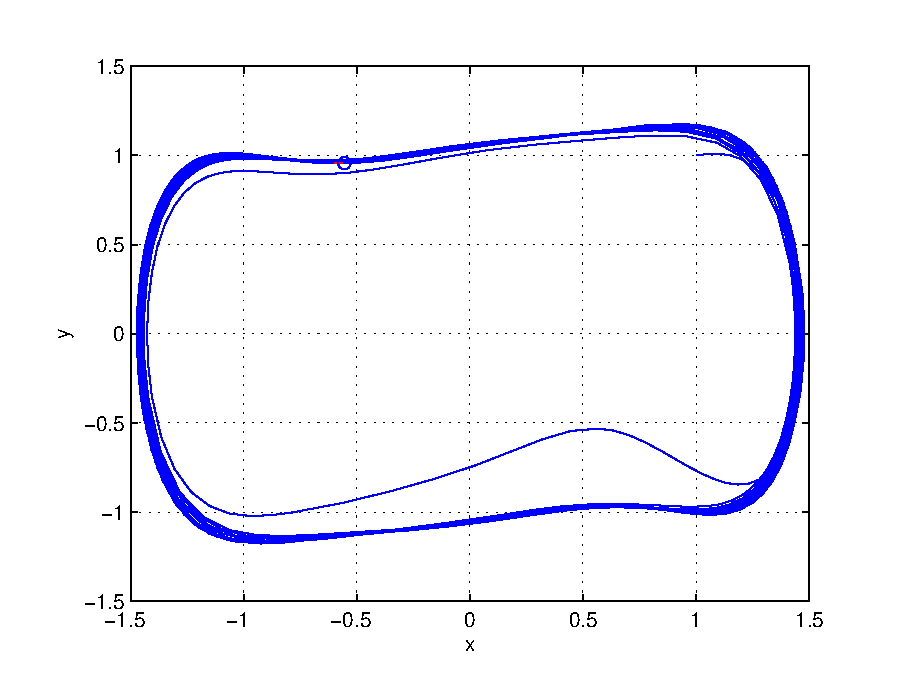
\includegraphics[width=1\linewidth]{duffing_sync.eps}}
	\caption{Фазовый портрет при ${\omega =\omega_{x}}$}
	\label{pic:duffing_sync}
\end{figure}
\begin{figure}[h]
	\center\scalebox{0.5}{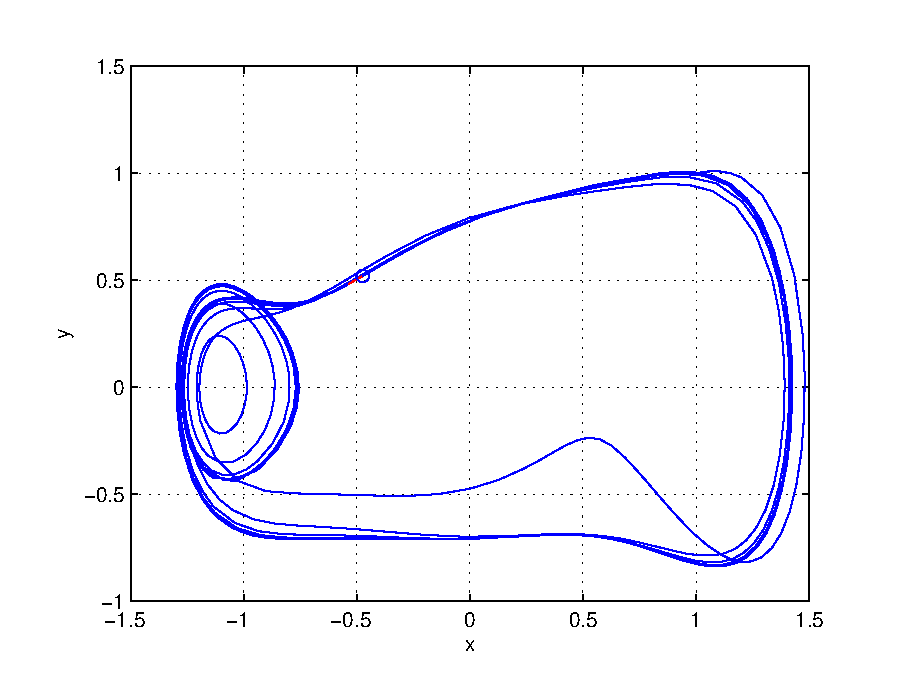
\includegraphics[width=1\linewidth]{duffing_chaos1.eps}}
	\caption{Фазовый портрет при ${\omega < \omega_{x}}$}
	\label{pic:duffing_chaos1}
\end{figure}
\begin{figure}[h]
	\center\scalebox{0.5}{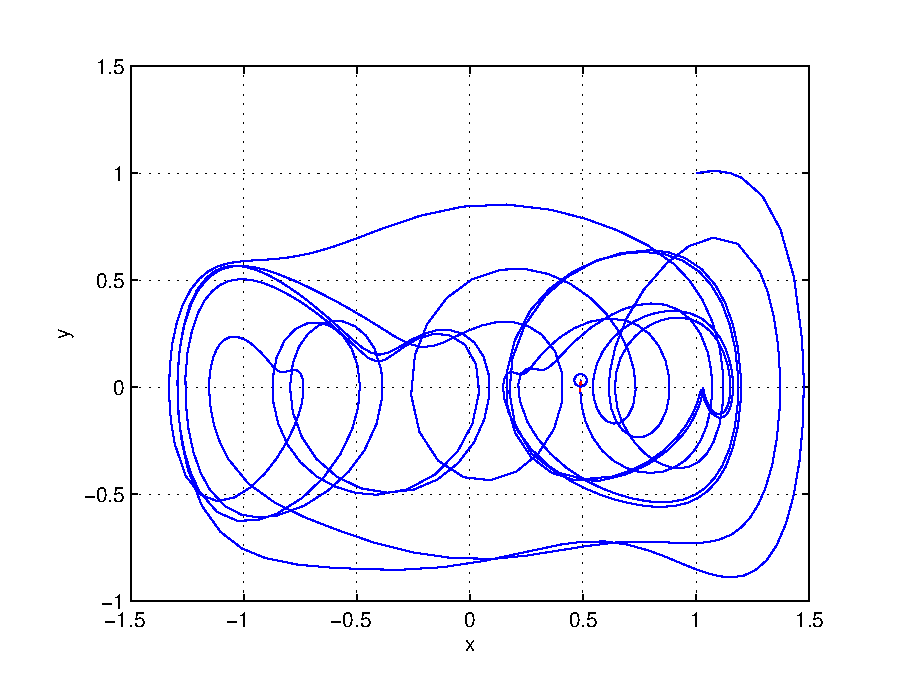
\includegraphics[width=1\linewidth]{duffing_chaos2.eps}}
	\caption{Фазовый портрет при ${\omega > \omega_{x}}$}
	\label{pic:duffing_chaos2}
\end{figure}
В качестве параметров уравнения применялись: $c = 0.5$, $\gamma=\gamma_{x}=0.36$, ${\omega=1}$

Часто для вычисления характеристик хаотической динамики применяется показатель Ляпунова.
Он показывает в каком состоянии находится система. Если система находится
в стабильном состоянии линии фазовой траектории будут близко прилегать одна к другой, в противном
случае система находится в состоянии хаоса. Детектор с применением показателя Ляпунова
представлен на Рис. \ref{pic:chaos_lyapunov}.
\begin{figure}[h]
	\center\scalebox{0.7}{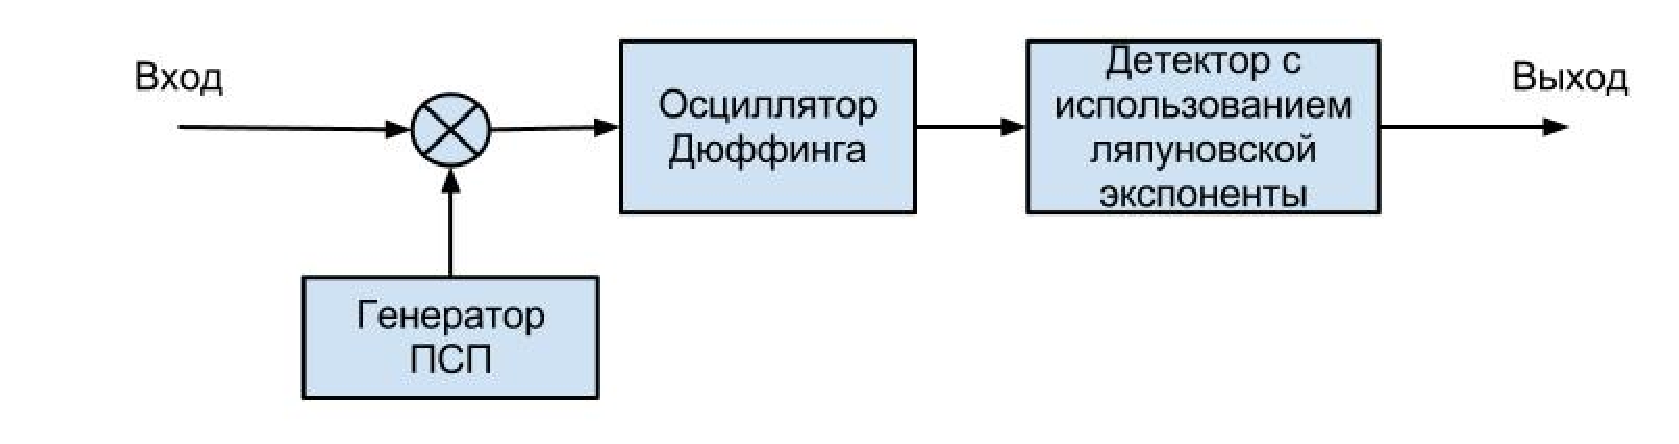
\includegraphics[width=1\linewidth]{Chaos_detector_Lyapunov.eps}}
	\caption{Схема детектора, основанного на показателе Ляпунова для осциллятора Дуффинга}
	\label{pic:chaos_lyapunov}
\end{figure}

В статье \cite{chaos_chen} предложен усовершенствованный метод, базирующийся на вычислении дисперсии
фазовой траектории. Действительно, на Рис. \ref{pic:duffing_sync}, \ref{pic:duffing_chaos1} и
\ref{pic:duffing_chaos2} видно, что когда система находится в хаотическом состоянии значение
дисперсии по координате ${x}$ больше, чем соответствующее значение в состоянии $\omega = \omega_{x}$.
На основе этого была предложена усовершенствованная схема детектора сигнала - Рис. \ref{pic:chaos_energy_detector}
\begin{figure}[h]
	\center\scalebox{0.7}{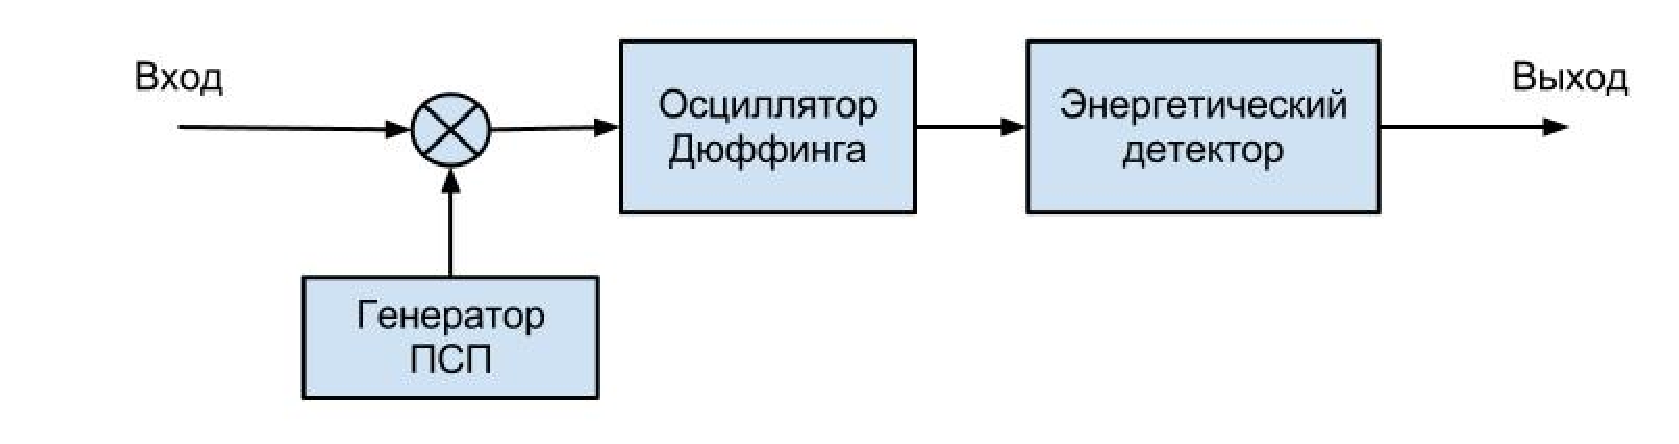
\includegraphics[width=1\linewidth]{chaos_detector.eps}}
	\caption{Схема энергетического детектора для осциллятора Дуффинга}
	\label{pic:chaos_energy_detector}
\end{figure}

В то же время, на данный момент никто не предложил цифровое представление осциллятора Дуффинга, а это затрудняет использование данного подхода
в реальных приемниках. Таким образом данное направление является в настоящее время больше теоретическим, чем практическим.

В работах \cite{hos_petropulu, hos_zhao} предложено использовать статистики высоких порядков для подавления шума и оценки
сигналов с низким уровнем ОСШ.

Интересная группа алгоритмов основывается на информационной избыточности ШПС, например, \cite{phd_che}. В данной
группе алгоритмов используется механизм появления нескольких точек на основном пике КФ, описанный в \cite{kaplan}. Пример
изображен на Рис. \ref{pic:sec1_peak_tcd}.
\begin{figure}[h]
	\center\scalebox{1}{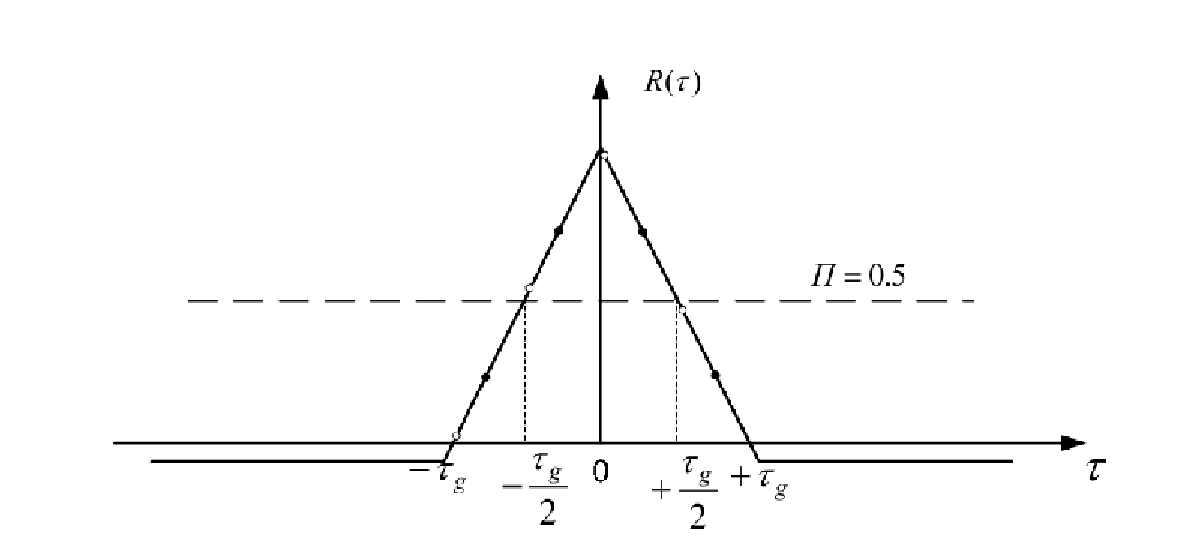
\includegraphics[width=1\linewidth]{corr_peak_tcd.eps}}
	\caption{Идеальная КФ ШПС с отмеченными точками возможного обнаружения}
	\label{pic:sec1_peak_tcd}
\end{figure}

На Рис. \ref{pic:sec1_peak_tcd} изображен пик КФ с несколькими точками. Две точки находятся выше порога ${\Pi=0.5}$.

в работе \cite{phd_che} рассмотрено создание субоптимального обнаружителя на основе информационной избыточности ШПС.
Получена целевая для системы синхронизации в целом и намечены дальнейшие пути развития данного направления.

Математический аппарат статистик высоких порядков (СВП или HOS - Higher-order statistics)
для исследования непричинных, причинных и нестабильных
(систем с не минимальной фазой) и негауссовых сигналов впервые был предложен в \cite{hos_petropulu} в 1993 году.
Этот метод позволяет не только подавлять цветной Гауссов шум, но также в некоторых случаях подавлять
цветной негауссов шум. В работе \cite{hos_zhao} был предложен метод оценки параметров ШПС с использованием СВП.

Более традиционные подходы оценке параметров ШПС сигналов с низким уровнем ОСШ рассмотрены в монографии \cite{ziedan-book}.
В данной монографии рассматриваются как методы детектирования и оценки параметров ШПС, основанные на когерентном накоплении, так и эффективные
системы слежения за частотой и фазой ПСП.

Так же публикуются работы по выбору порога в алгоритмах захвата ШПС. Например, в работах \cite{2max_ieee, 2max_article} представлен алгоритм
\textquotedblleft{Peak-finding algorithm}\textquotedblright,
в данной работе введем перевод -
\textquotedblleft{Алгоритм нахождения пика}\textquotedblright (АНП). 

Предложенный в работах алгоритм можно разбить на несколько шагов:
\begin{itemize}
	\item[Шаг 1] Подсчитать КФ, используя БПФ.
	\item[Шаг 2] Найти главный пик КФ, найти второй пик КФ, найти среднее значение КФ.
	\item[Шаг 3] Нормализовать полученные значения относительно главного пика КФ.
	\item[Шаг 4] Если (максимум КФ - среднее) > ${\Pi_1}$ и (максимум КФ - 
		второй максимум КФ) > ${\Pi_2}$, тогда принимается решение о наличии сигнала в принимаемой смеси. 
\end{itemize}

В статье авторов \cite{2max_ieee} предложены следующие значения для порогов:
${\Pi_1} = 0.3$ дБ и  ${\Pi_2} = 0.15$ дБ. Так же авторы предлагают итерационную процедуру для нахождения фазы ПСП и частоты смещения ДОПЛЕра:
\begin{itemize}
	\item[Шаг 1] Начать вычисление с 1 мс.
	\item[Шаг 2] Получить результаты АНП.
	\item[Шаг 3] Если фаза ПСП и частота не могут быть найдены, увеличить время интегрирования сигнала.
		Использовать следующие значения для интегрирования: 1мс -> 10мс -> 50мс -> 100мс -> 200мс -> 500мс -> 1000мс
\end{itemize}

%%%%%%%%
{\bf{Цель и задачи диссертации}}

Целью диссертационной работы является разработка и анализ алгоритмов оценки информационных параметров сигнала в системах с кодовым разделением каналов на основе
параметрического метода оценки частоты на фоне аддитивного белого гауссового шума и интерференционной помехи,
с возможностью реализации на современной элементной базе.

Для достижения поставленной цели в диссертации решаются следующие задачи:
\begin{enumerate}
	\item {С использованием методов параметрической идентификации автором разработан алгоритм оценки информационных параметров для одного источника сигнала
		в CDMA-системах на фоне аддитивного белого гауссового шума.}
	\item {Адаптация алгоритма повышения отношения сигнал/шум при оценке автокорреляционной функции гармонического сигнала для использования при обработке
		CDMA-сигнала в приемниках реального времени.}
	\item {Разработка комплексированного алгоритма оценки информационных параметров CDMA-сигнала на фоне аддитивного белого гауссового шума и
		интерференционной помехи, основанный на алгоритме Delay and Multiply Approach, алгоритме повышения сигнал/шум в оценке автокорреляционной функции 
		и авторегрессионной модели второго порядка.}
	\item {Сравнительный анализ разработанных алгоритмов с типовыми решениями в области оценки информационных параметров сигнала используемых в CDMA-системах.}
	\item {Полунатурное моделирование с использованием оригинальной аппаратной платформы на реальных данных CDMA-системы Navstar GPS.}
\end{enumerate}

{\bf{Научная новизна результатов}}
\begin{enumerate}
	\item{На основе теории параметрической идентификации автором разработан алгоритм оценки информационных параметров сигнала в системах с кодовым разделением каналов.}
	\item{Предложен алгоритм компенсации окрашенного шума на основе итеративного вычисления автокорреляционной функции для
		получения несмещенной оценки частоты с использованием параметрического метода оценки спектра.}
	\item{Предложен способ эффективного итеративного вычисления автокорреляционной функции в базисе Фурье для использования в
		приемниках реального времени.}
	\item{Предложен способ комплексирования алгоритмов оценки фазы псевдослучайной последовательности (ПСП) Delay And Multiply Approach, алгоритма итеративной оценки АКФ и
		параметрического метода оценки спектра в задаче оценки параметров сигнала с расширенным спектром.}
\end{enumerate}

{\bf{Практическая ценность}}
\begin{enumerate}
	\item {Усовершенствован алгоритм повышения отношения сигнал/шум при оценке автокорреляционной функции. Оптимизация вычислительных затрат позволяет использовать
		данный алгоритм в приемниках реального времени.}
	\item {Комплексированный алгоритм оценки информационных параметров CDMA-сигнала позволяет существенно снизить вычислительные затраты.}
	\item {Программно-аппаратный стенд для экспериментального исследования систем цифровой связи с использованием технологии CDMA,
		позволяет подтвердить схемотехническую реализуемость разработанных алгоритмов.}
\end{enumerate}

{\bf{Апробация результатов}}

Результаты диссертации прошли апробацию на:
\begin{enumerate}
	\item 7-ой Всероссийской конференции «Радиолокация и радиосвязь» (Москва 2013 г.);
	\item Международной конференции «Радиоэлектронные устройства и системы для инфокоммУникационных технологий - РЕС-2013» (Москва 2013 г.);
	\item V Международной студенческой научно-практической конференции «Интеллектуальный потенциал XXI века: ступени познания» (Новосибирск 2011 г.).
\end{enumerate}

{\bf{Внедрение результатов работы:}}
\begin{enumerate}
	\item Результаты диссертации использованы в НИОКР ЗАО «Телум», что подтверждено актом о внедрении.
	\item Результаты диссертации использованы в учебном процессе на кафедре автономных информационных и управляющих систем МГТУ им. Н.Э. Баумана,
		что подтверждено актом об использовании и кафедре "Управление и моделирование систем" Московского Государственного Университета Приборостроения
		и Информатики, что подтверждено актом об использовании.
\end{enumerate}

{\bf{Объем и структура диссертации}}

Диссертация состоит из введения, четырех глав, заключения и списка литературы. Общий объем составляет 138 страниц, включающих 24 страниц приложения, 52 иллюстраций,
X таблицы и список литературы из 62 наименований.

{\bf{Положения, выносимые на защиту}}
\begin{enumerate}
	\item {Алгоритм оценки информационных параметров CDMA-сигнала на фоне белого шума на основе АР-модели принимаемого сигнала.}
	\item {Алгоритм повышения отношения сигнал шум и подавления интерференционной помехи применительно к задаче оценки информационных параметров CDMA-сигнала.}
	\item {Алгоритм оценки информационных параметров CDMA-сигнала на фоне интерференционной помехи и шума на основе алгоритмов: Delay and Multiply Approach,
		усовершенствованного алгоритма итеративного вычисления автокорреляционной функции и АР-модели принимаемого сигнала.}
	\item {Результаты анализа точности, вычислительных затрат разработанных алгоритмов, а также сравнительный анализ с типовым алгоритмом.}
\end{enumerate}

%%%%%%
\clearpage
 % введение

\addcontentsline{toc}{section}{СПИСОК СОКРАЩЕНИЙ}
\section*{СПИСОК СОКРАЩЕНИЙ}
АБГШ - аддитивный белый гауссовский шум				\\
АКФ – автокорреляционная функция				\\
АР - авторегрессия						\\
АРСС - авторегрессия скользящего среднего			\\
ДПФ - дискретное преобразование Фурье				\\
ДФМ - двоичная фазовая манипуляция				\\
ОСШ - отношение сигнал-шум 					\\
СНРС - сигналы спутниковых радионавигационных систем		\\
СНС - спутниковая навигационная система				\\
CC - скользящее среднее						\\
ПСП – псевдослучайная последовательность			\\
ФАПЧ - фазовая автоподстройка частоты				\\
ШПС -  широкополосные сигналы (шумоподобные сигналы)		\\
\newpage
		% acronyms 
\addcontentsline{toc}{section}{СПИСОК УСЛОВНЫХ ОБОЗНАЧЕНИЙ}
\section*{СПИСОК УСЛОВНЫХ ОБОЗНАЧЕНИЙ}
${M[X]}$ - математическое ожидание случайной величины $X$	\\
${D[X]}$ - дисперсия случайной величины $X$			\\
\newpage
		% definitions

\addcontentsline{toc}{chapter}{Введение}
\chapter*{Введение}

Большое количество современных систем являются беспроводными. Простота развертывания, мобильность, относительно низкая
стоимость, вот основные преимущества беспроводных систем. Количество мобильных устройств (телефоны, планшетные компьютеры
и т.д.) с каждым годом стремительно растет, только мобильных телефонов в 2011 году было 5.6 миллиарда и покрывало 79.86\%
\cite{wiki_mobilenum} населения земли. Технологии беспроводной связи глубоко проникли во все сферы жизни общества:
обеспечение безопасности с помощью RFID датчиков, предоставление доступа в интернет по технологиями 3G, Wi-Fi, 
сотовая связь по различным технологиям (GSM, CDMA, DAMPS). Некоторые из этих систем строятся на основе методики
расширения спектра, которая отвечает современным требованиям по мощности сигнала, а также по безопасности передаваемых
данных. В основе таких систем лежат шумоподобные (широкополосные) сигналы - ШПС. Вместе с тем растут требования к таким
системам. Применение ШПС ставит ряд специфических задач по обработке информации, обусловленных особенностями ШПС.
Свойства характерные для ШПС, выгодно отличают данный класс систем от класса узкополосных систем, но с другой стороны
оборачивается усложнением методов обработки ШПС.

Внедрение новых технологий требует увеличение полосы частот. Разнообразие технологий беспроводной передачи данных среди
гражданских и военных систем ведет к перегрузке каналов связи и все более высоким требованиям к скорости передачи
данных. С учётом данных требований применение систем передачи информации с ШПС становится все более востребованным.

Принимая во внимание географические размеры России и стратегическую важность обладания собственными системами спутникового
позиционирования, правительство Российский Федерации уделяет особое внимание разработке собственной системы
глобального спутникового позиционирования ГЛОНАСС. Обладание собственными технологиями системы спутниковой навигации (СНС), государство может обезопасить
себя в случае военных конфликтов от ограничения применения американской системы СНС Navstar GPS в зоне конфликта.

Разработка систем, позволяющих работать с несколькими различными СНС, позволит повысить точность определения координат
в сложных условиях города. Сложность детектирования сигнала и определения координат обусловлена наличием плотной
застройки многоэтажными зданиями. В городских условиях задача подавления интерференционной помехи становится особенно
актуальной. Спектр интерференционной помехи не является белым, а фильтрация и компенсация цветного шума
требует разработки специальных алгоритмов.

Новые цифровые процессоры позволяют применять подходы, которые еще 10-15 лет назад были бесперспективными.
В данной работе развиваются подходы на основе построения параметрической модели ШПС. Невозможность использования
методов требующих вычислений с высокой точностью в приемниках реального времени
10-15 лет назад была обусловлена слабой производительностью процессоров и микроконтроллеров, а также существенной
стоимостью процессоров с модулем для операций с числами с плавающей точкой. Современное развитие цифровых технологий делает 
возможным применение параметрических методов оценки спектра взамен традиционного подхода основанного на непараметрического
анализа спектра.

Основа теории систем связи с ШПС была заложена в работах В.А. Котельникова и К. Шеннона.
России в этой области занимаются В.И. Борисов, В.Б. Пестряков, В.И. Журавлев, М.И. Жодзишский, Б.И. Шахтарин, Л.Е.  Варакин, В.Е. Гантмахер и др.

Изначально методы расширенного спектра применялись при разработке военных систем управления и связи \cite{sklyar}.
К концу второй мировой войны расширение спектра применялось в радиолокации для борьбы с преднамеренными помехами, а
в последствии развитие данной технологии объяснялось желанием создать помехоустойчивые системы связи.
В конце 40-х-начале 50-х годов прошлого века Мортимер Рогофф, сотрудник Международной Телефонной и Телеграфной Корпорации (США) (ITT),
провёл эксперимент по передаче информации при помощи псевдошумового сигнала \cite{sklyar}, среди отечественных ученых
в середине 30-х годов прошлого века работу об основах кодового разделения каналов написал Д.В. Агеев.
Первые разработки таких систем относились к военным отраслям. Данный факт объясняется рядом особенностей, которыми обладают
сигналы с расширенным спектром, в числе которых — сложность перехвата заложенной в них информации,
высокая помехоустойчивость, а также трудность обнаружения факта работы передатчика. В процессе исследований расширенному спектру
нашлось и другое применение - снижение плотности энергии, высокоточная локация, использование при множественном доступе
\cite{sklyar}

Системы связи с широкополосными сигналами занимают особое место. Их особенные свойства выделяют данный класс из других систем
связи. Высокая помехозащищенность при действии сильной помехи, кодовое разделение большого количества абонентов, прием
информации с высокой достоверностью - отличительные особенности широкополосных система. Эти черты были известно, но
уровень элементной базы и низкий уровень помех не позволяли получить развития системам данного класса. Однако развитие
элементной привело к широкому распространению данного вида сигналов. В настоящее они применяются в системах спутниковой навигации,
системах сотовой связи и др \cite{varakin-book}.

Отношение сигнал/шум (ОСШ) на входе приемника может быть очень низким. Для обеспечения высокой помехозащищенности 
в таких случаях используются ШПС с большими и сверхбольшими базами.

К созданию сложных широкополосных сигналов (СШС) привело решение ряда проблем при развитии систем передачи данных.
Первая проблема встала при разработке новых радиолокационных система. Для дальнейшего развития требовалось
решить несколько противоречий: требование высокой разрешающей способности по дальности и дальностью обнаружения
целей в импульсных РЛС, требование точного измерения скорости и высокое разрешение по дальности, требование
увеличить дальность при ограничении пиковой мощности \cite{gantmaher-book}. Решение данных задач было предложено
Ф. Вудвардом. Им было показано, что дополнительным параметром является форма сигнала. Длительность сигнала
может быть больше - настолько больше, насколько это необходимо для обеспечения энергетических требований, а требование
разрешения по дальности и точности измерений определяются шириной полосы сигнала. Данные требования обеспечивается
путем сжатия импульса на стороне приемника. Вудворд сформулировал принципы: произведение эффективной полосы частот
радиосигнала на его длительность должен быть существенно больше единиц ${FT>>1}$, внутренняя структура сигнала
должна быть такой, чтобы обеспечить возможность приемнику сжатие распределенного во времени сигнала в короткий импульс,
соответствующий полосе ${F}$ \cite{gantmaher-book}.

В \cite{gantmaher-book} показана связь пропускной способности канала с понятием ШПС. При ${R_e<<1}$ можно записать:
\begin{equation}
	%\label{eq:shennon_cdma}
	FT = \frac{1}{\log(1+R_e)}, \nonumber
\end{equation}
где ${R_e}$ - ОСШ, ${F}$ - эффективная полоса частот, ${T}$ - длительность.

Стоить отметить, что при ${R_e<<1}$, левая часть данного выражения стремится к бесконечности, а значит
ШПС позволяет обеспечить теоретически неограниченную достоверность передачи информации. Второе важное свойство
ШПС - способность работать "под шумами". Что обеспечивает скрытность
передачи информации, а с другой высокую степень уплотнения каналов связи и, как следствие, решение современных проблем
с перегруженностью каналов связи.

В данной работе будет рассматриваться ШПС модулированный ПСП на основе двоичной рекуррентной последовательности.
Для выделения данных из потока необходимо иметь точно синхронизированную копию ПСП, которая была использована
при модулировании сигнала на передающей стороне. Для достижения синхронизма на стороне приемника необходимо
устранить неопределенность в двух областях: неопределенность по частоте и неопределенность по фазе (задержке) ПСП.
Неопределенность по фазе ПСП обусловлена неопределенностью в расстоянии между передатчиком и приемником. Неопределенность
по частоте обусловлена в первую очередь доплеровским эффектом, а также нестабильностью опорных генераторов в
передатчике и приемнике. После устранения неопределенности по частоте для достижения точной синхронизации
начинается процесс слежения за частотой. Неопределенность по фазе ПСП устранить, не используя полный перебор,
невозможно в силу корреляционных свойств ПСП. Таким образом можно заключить, что задача быстрого и эффективного
поиска и оценки параметров ШПС является актуальной.

В данной работе рассматривается подход программного приемника (Software Defined Receiver - SDR)
\cite{akos-book, grayver-book, pany-book} для оценки параметров ШПС. Как уже было отражено выше, ШПС применяется во
многих системах. В данной работе для полунатурного эксперимента будет рассматриваться сигнал СНС Navstar GPS. Данная система передачи 
информации (СПИ) использует ПСП Голда \cite{gold-ieee} для модулирования сигнала.

Традиционные подходы к реализации приемника СНС Navstar GPS отражены в \cite{akos-book, tsui}. 

Популярность и распространенность данной системы стимулирует исследования в области детектирования
и оценки параметров ШПС сигнала.

Существуют исследования в области применения теории хаоса - детектирование и оценка
частоты ШПС с применением осциллятора Дуффинга \cite{chaos_cambridge, chaos_chen, chaos_huang, chaos_wang}. Преимуществом
данного подхода является то, что свойства осциллятора позволяют детектировать сигналы с экстремально низким ОСШ.

Осциллятор Дуффинга с гармоническим внешним воздействием может быть описан уравнением:
\begin{equation}
	\label{eq:duffing}
	mx'' + cx' + k_{1}x + k_{2}x^3 = F_{0}\cos(\omega{t}),
\end{equation}
где $m$ - масса, $c$ - коэффициент диссипации, $x$ - состояние осциллятора, $k_1$ и $k_2$ - линейный и нелинейный коэффициенты соответственно,
$F_{0}\cos(\omega{t})$ - внешнее воздействие.

Подробно уравнение \ref{eq:duffing} рассмотрено в \cite{chaos_neimark_landa}.
Для использования осциллятора Дуффинга с целью оценки параметров ШПС была предложена усовершенствованная форма \cite{chaos_song, chaos_chen}:
\begin{equation}
	\label{eq:duffing_gps}
	x'' +cx' - x^3 + x^5 = \gamma\cos(\omega{t}) + (\gamma_{x}\cos(\omega_{x}) + n(t))
\end{equation}

Можно переписать динамическую систему \ref{eq:duffing_gps} в виде:
\begin{equation}
	\label{eq:duffing_gps_2}
	\left\{
	\begin{aligned}
		y(t) & = x'(t) \\
		y'(t) & =  -cx' + x^3 - x^5 + \gamma\cos(\omega{t}) + (\gamma_{x}\cos(\omega_{x}) + n(t)),
	\end{aligned}
	\right.
\end{equation}
где ${n(t)}$ - аддитивный белый гауссовский шум (АБГШ), имеющий нулевое среднее  значение и КФ ${R_n(\tau) = \frac{N_0}{2} \delta(\tau)}$,
а ${N_0}$ - односторонний энергетический спектр.

Пример фазового портрета при ${\omega=\omega_{x}}$ изображен на Рис. \ref{pic:duffing_sync},
фазовый портрет хаоса расположен на Рис. \ref{pic:duffing_chaos1}, Рис. \ref{pic:duffing_chaos2}
\begin{figure}[h]
	\center\scalebox{0.5}{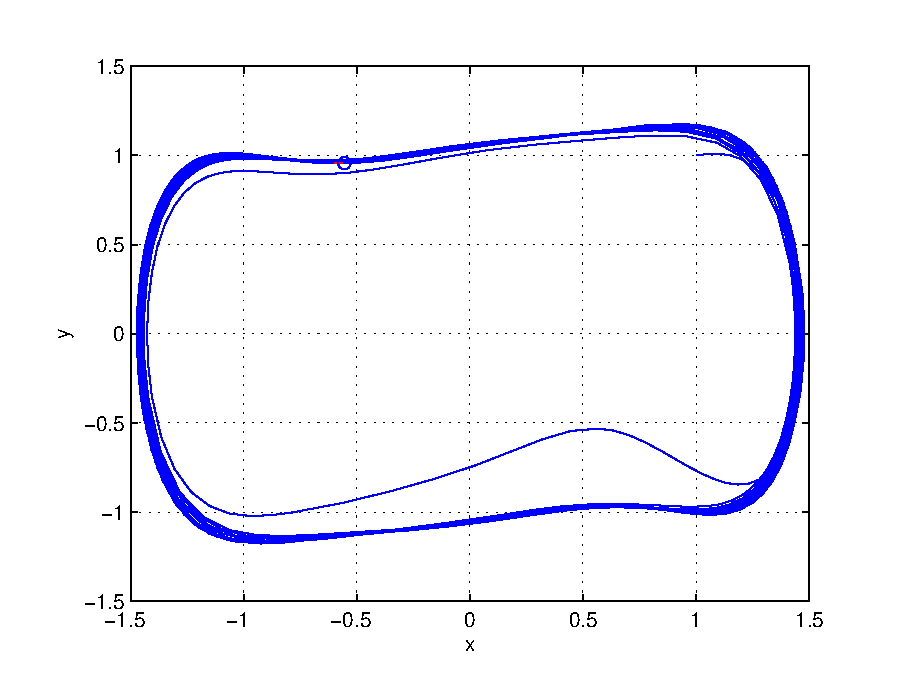
\includegraphics[width=1\linewidth]{duffing_sync.eps}}
	\caption{Фазовый портрет при ${\omega =\omega_{x}}$}
	\label{pic:duffing_sync}
\end{figure}
\begin{figure}[h]
	\center\scalebox{0.5}{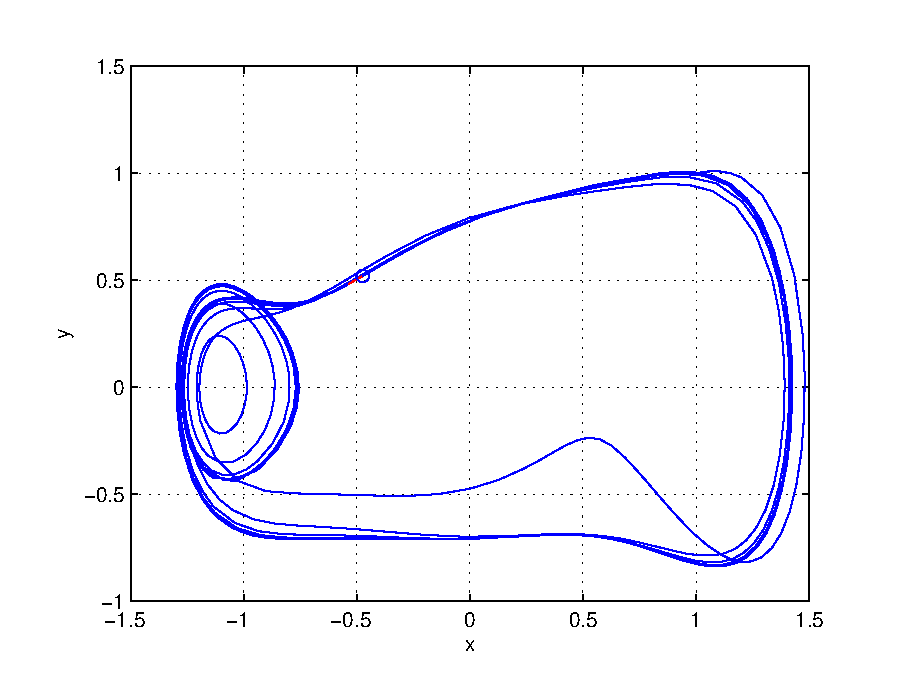
\includegraphics[width=1\linewidth]{duffing_chaos1.eps}}
	\caption{Фазовый портрет при ${\omega < \omega_{x}}$}
	\label{pic:duffing_chaos1}
\end{figure}
\begin{figure}[h]
	\center\scalebox{0.5}{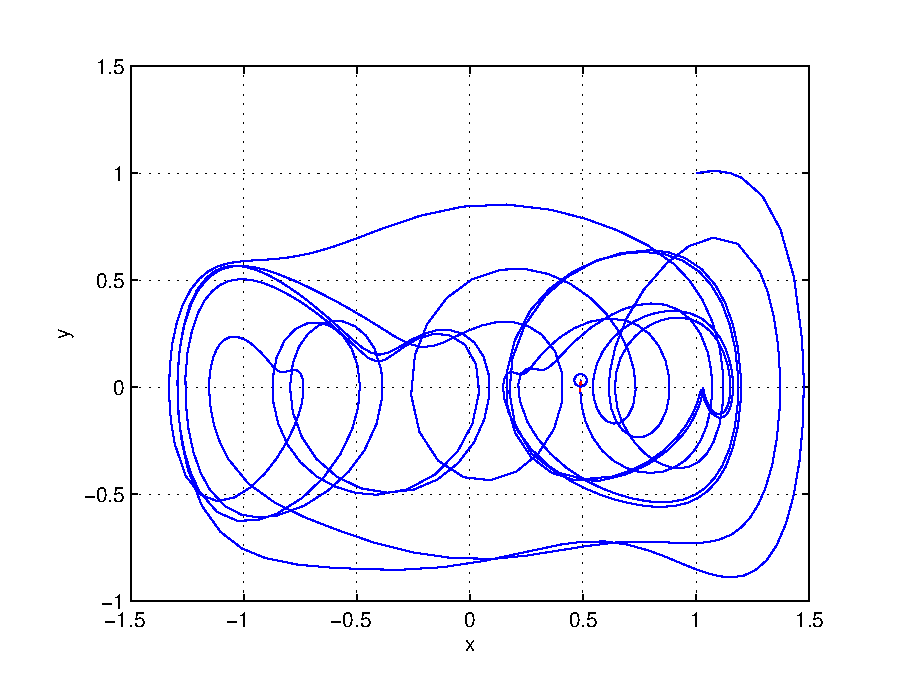
\includegraphics[width=1\linewidth]{duffing_chaos2.eps}}
	\caption{Фазовый портрет при ${\omega > \omega_{x}}$}
	\label{pic:duffing_chaos2}
\end{figure}
В качестве параметров уравнения применялись: $c = 0.5$, $\gamma=\gamma_{x}=0.36$, ${\omega=1}$

Часто для вычисления характеристик хаотической динамики применяется показатель Ляпунова.
Он показывает в каком состоянии находится система. Если система находится
в стабильном состоянии линии фазовой траектории будут близко прилегать одна к другой, в противном
случае система находится в состоянии хаоса. Детектор с применением показателя Ляпунова
представлен на Рис. \ref{pic:chaos_lyapunov}.
\begin{figure}[h]
	\center\scalebox{0.7}{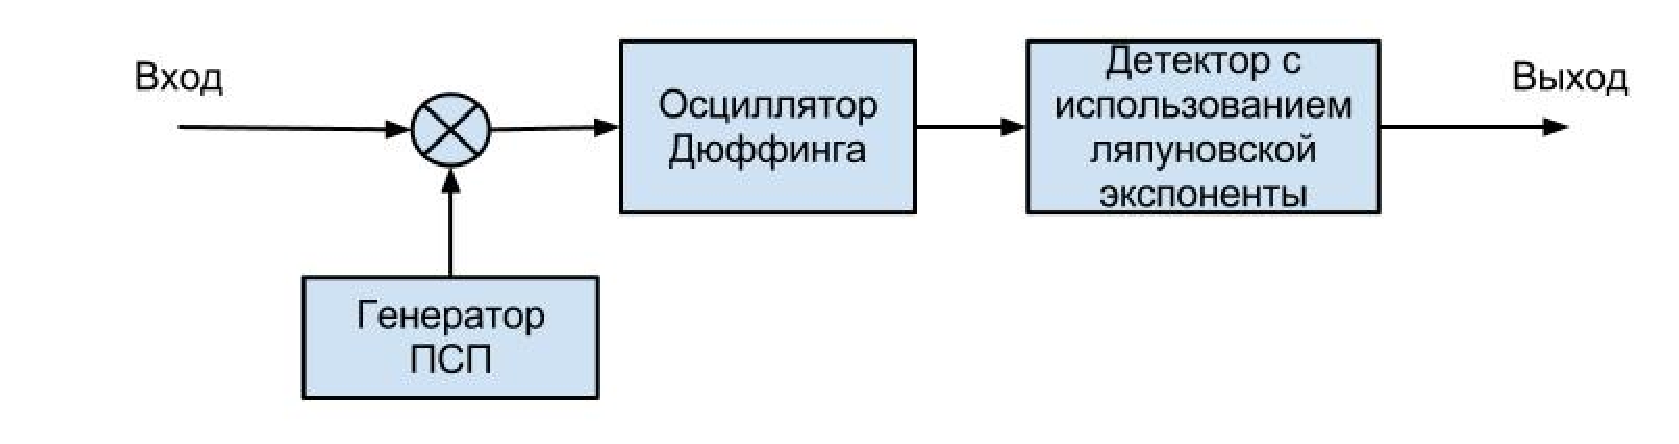
\includegraphics[width=1\linewidth]{Chaos_detector_Lyapunov.eps}}
	\caption{Схема детектора, основанного на показателе Ляпунова для осциллятора Дуффинга}
	\label{pic:chaos_lyapunov}
\end{figure}

В статье \cite{chaos_chen} предложен усовершенствованный метод, базирующийся на вычислении дисперсии
фазовой траектории. Действительно, на Рис. \ref{pic:duffing_sync}, \ref{pic:duffing_chaos1} и
\ref{pic:duffing_chaos2} видно, что когда система находится в хаотическом состоянии значение
дисперсии по координате ${x}$ больше, чем соответствующее значение в состоянии $\omega = \omega_{x}$.
На основе этого была предложена усовершенствованная схема детектора сигнала - Рис. \ref{pic:chaos_energy_detector}
\begin{figure}[h]
	\center\scalebox{0.7}{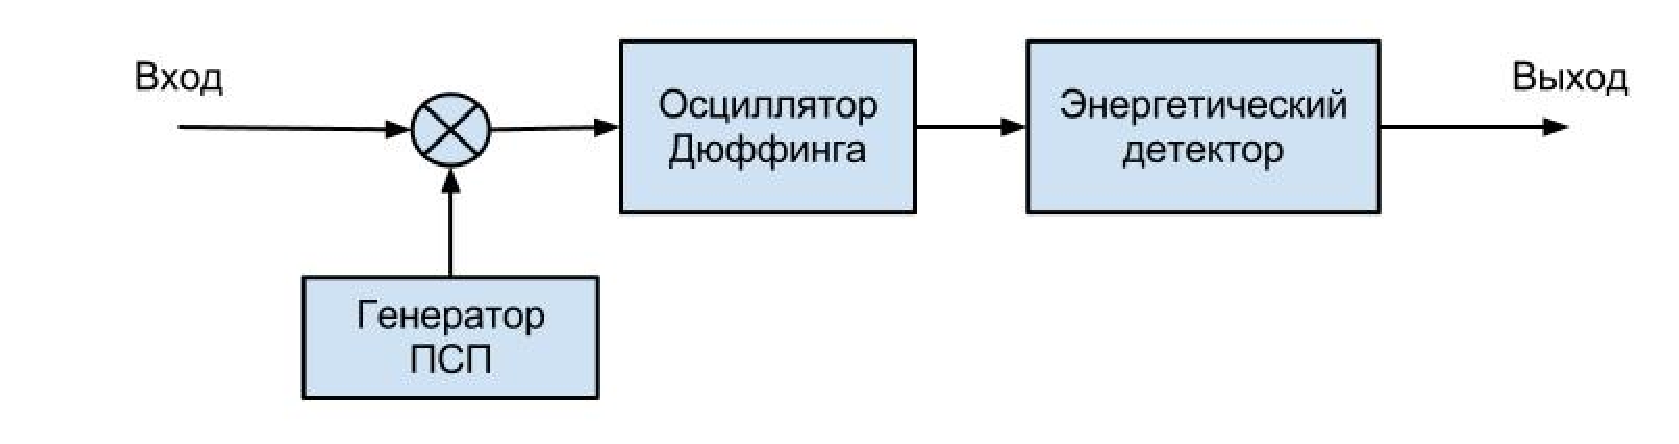
\includegraphics[width=1\linewidth]{chaos_detector.eps}}
	\caption{Схема энергетического детектора для осциллятора Дуффинга}
	\label{pic:chaos_energy_detector}
\end{figure}

В то же время, на данный момент никто не предложил цифровое представление осциллятора Дуффинга, а это затрудняет использование данного подхода
в реальных приемниках. Таким образом данное направление является в настоящее время больше теоретическим, чем практическим.

В работах \cite{hos_petropulu, hos_zhao} предложено использовать статистики высоких порядков для подавления шума и оценки
сигналов с низким уровнем ОСШ.

Интересная группа алгоритмов основывается на информационной избыточности ШПС, например, \cite{phd_che}. В данной
группе алгоритмов используется механизм появления нескольких точек на основном пике КФ, описанный в \cite{kaplan}. Пример
изображен на Рис. \ref{pic:sec1_peak_tcd}.
\begin{figure}[h]
	\center\scalebox{1}{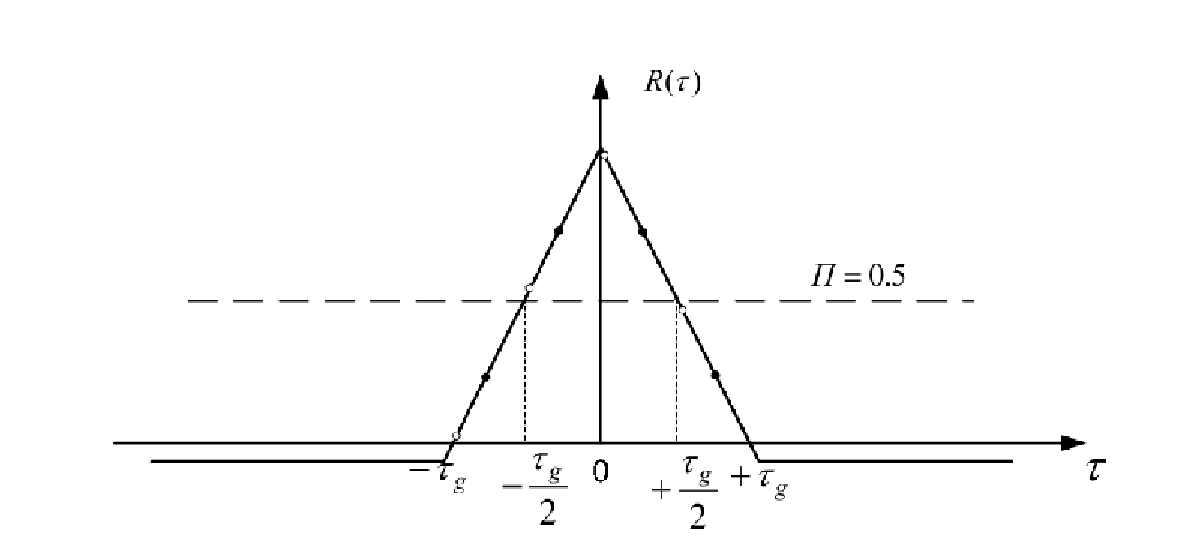
\includegraphics[width=1\linewidth]{corr_peak_tcd.eps}}
	\caption{Идеальная КФ ШПС с отмеченными точками возможного обнаружения}
	\label{pic:sec1_peak_tcd}
\end{figure}

На Рис. \ref{pic:sec1_peak_tcd} изображен пик КФ с несколькими точками. Две точки находятся выше порога ${\Pi=0.5}$.

в работе \cite{phd_che} рассмотрено создание субоптимального обнаружителя на основе информационной избыточности ШПС.
Получена целевая для системы синхронизации в целом и намечены дальнейшие пути развития данного направления.

Математический аппарат статистик высоких порядков (СВП или HOS - Higher-order statistics)
для исследования непричинных, причинных и нестабильных
(систем с не минимальной фазой) и негауссовых сигналов впервые был предложен в \cite{hos_petropulu} в 1993 году.
Этот метод позволяет не только подавлять цветной Гауссов шум, но также в некоторых случаях подавлять
цветной негауссов шум. В работе \cite{hos_zhao} был предложен метод оценки параметров ШПС с использованием СВП.

Более традиционные подходы оценке параметров ШПС сигналов с низким уровнем ОСШ рассмотрены в монографии \cite{ziedan-book}.
В данной монографии рассматриваются как методы детектирования и оценки параметров ШПС, основанные на когерентном накоплении, так и эффективные
системы слежения за частотой и фазой ПСП.

Так же публикуются работы по выбору порога в алгоритмах захвата ШПС. Например, в работах \cite{2max_ieee, 2max_article} представлен алгоритм
\textquotedblleft{Peak-finding algorithm}\textquotedblright,
в данной работе введем перевод -
\textquotedblleft{Алгоритм нахождения пика}\textquotedblright (АНП). 

Предложенный в работах алгоритм можно разбить на несколько шагов:
\begin{itemize}
	\item[Шаг 1] Подсчитать КФ, используя БПФ.
	\item[Шаг 2] Найти главный пик КФ, найти второй пик КФ, найти среднее значение КФ.
	\item[Шаг 3] Нормализовать полученные значения относительно главного пика КФ.
	\item[Шаг 4] Если (максимум КФ - среднее) > ${\Pi_1}$ и (максимум КФ - 
		второй максимум КФ) > ${\Pi_2}$, тогда принимается решение о наличии сигнала в принимаемой смеси. 
\end{itemize}

В статье авторов \cite{2max_ieee} предложены следующие значения для порогов:
${\Pi_1} = 0.3$ дБ и  ${\Pi_2} = 0.15$ дБ. Так же авторы предлагают итерационную процедуру для нахождения фазы ПСП и частоты смещения ДОПЛЕра:
\begin{itemize}
	\item[Шаг 1] Начать вычисление с 1 мс.
	\item[Шаг 2] Получить результаты АНП.
	\item[Шаг 3] Если фаза ПСП и частота не могут быть найдены, увеличить время интегрирования сигнала.
		Использовать следующие значения для интегрирования: 1мс -> 10мс -> 50мс -> 100мс -> 200мс -> 500мс -> 1000мс
\end{itemize}

%%%%%%%%
{\bf{Цель и задачи диссертации}}

Целью диссертационной работы является разработка и анализ алгоритмов оценки информационных параметров сигнала в системах с кодовым разделением каналов на основе
параметрического метода оценки частоты на фоне аддитивного белого гауссового шума и интерференционной помехи,
с возможностью реализации на современной элементной базе.

Для достижения поставленной цели в диссертации решаются следующие задачи:
\begin{enumerate}
	\item {С использованием методов параметрической идентификации автором разработан алгоритм оценки информационных параметров для одного источника сигнала
		в CDMA-системах на фоне аддитивного белого гауссового шума.}
	\item {Адаптация алгоритма повышения отношения сигнал/шум при оценке автокорреляционной функции гармонического сигнала для использования при обработке
		CDMA-сигнала в приемниках реального времени.}
	\item {Разработка комплексированного алгоритма оценки информационных параметров CDMA-сигнала на фоне аддитивного белого гауссового шума и
		интерференционной помехи, основанный на алгоритме Delay and Multiply Approach, алгоритме повышения сигнал/шум в оценке автокорреляционной функции 
		и авторегрессионной модели второго порядка.}
	\item {Сравнительный анализ разработанных алгоритмов с типовыми решениями в области оценки информационных параметров сигнала используемых в CDMA-системах.}
	\item {Полунатурное моделирование с использованием оригинальной аппаратной платформы на реальных данных CDMA-системы Navstar GPS.}
\end{enumerate}

{\bf{Научная новизна результатов}}
\begin{enumerate}
	\item{На основе теории параметрической идентификации автором разработан алгоритм оценки информационных параметров сигнала в системах с кодовым разделением каналов.}
	\item{Предложен алгоритм компенсации окрашенного шума на основе итеративного вычисления автокорреляционной функции для
		получения несмещенной оценки частоты с использованием параметрического метода оценки спектра.}
	\item{Предложен способ эффективного итеративного вычисления автокорреляционной функции в базисе Фурье для использования в
		приемниках реального времени.}
	\item{Предложен способ комплексирования алгоритмов оценки фазы псевдослучайной последовательности (ПСП) Delay And Multiply Approach, алгоритма итеративной оценки АКФ и
		параметрического метода оценки спектра в задаче оценки параметров сигнала с расширенным спектром.}
\end{enumerate}

{\bf{Практическая ценность}}
\begin{enumerate}
	\item {Усовершенствован алгоритм повышения отношения сигнал/шум при оценке автокорреляционной функции. Оптимизация вычислительных затрат позволяет использовать
		данный алгоритм в приемниках реального времени.}
	\item {Комплексированный алгоритм оценки информационных параметров CDMA-сигнала позволяет существенно снизить вычислительные затраты.}
	\item {Программно-аппаратный стенд для экспериментального исследования систем цифровой связи с использованием технологии CDMA,
		позволяет подтвердить схемотехническую реализуемость разработанных алгоритмов.}
\end{enumerate}

{\bf{Апробация результатов}}

Результаты диссертации прошли апробацию на:
\begin{enumerate}
	\item 7-ой Всероссийской конференции «Радиолокация и радиосвязь» (Москва 2013 г.);
	\item Международной конференции «Радиоэлектронные устройства и системы для инфокоммУникационных технологий - РЕС-2013» (Москва 2013 г.);
	\item V Международной студенческой научно-практической конференции «Интеллектуальный потенциал XXI века: ступени познания» (Новосибирск 2011 г.).
\end{enumerate}

{\bf{Внедрение результатов работы:}}
\begin{enumerate}
	\item Результаты диссертации использованы в НИОКР ЗАО «Телум», что подтверждено актом о внедрении.
	\item Результаты диссертации использованы в учебном процессе на кафедре автономных информационных и управляющих систем МГТУ им. Н.Э. Баумана,
		что подтверждено актом об использовании и кафедре "Управление и моделирование систем" Московского Государственного Университета Приборостроения
		и Информатики, что подтверждено актом об использовании.
\end{enumerate}

{\bf{Объем и структура диссертации}}

Диссертация состоит из введения, четырех глав, заключения и списка литературы. Общий объем составляет 138 страниц, включающих 24 страниц приложения, 52 иллюстраций,
X таблицы и список литературы из 62 наименований.

{\bf{Положения, выносимые на защиту}}
\begin{enumerate}
	\item {Алгоритм оценки информационных параметров CDMA-сигнала на фоне белого шума на основе АР-модели принимаемого сигнала.}
	\item {Алгоритм повышения отношения сигнал шум и подавления интерференционной помехи применительно к задаче оценки информационных параметров CDMA-сигнала.}
	\item {Алгоритм оценки информационных параметров CDMA-сигнала на фоне интерференционной помехи и шума на основе алгоритмов: Delay and Multiply Approach,
		усовершенствованного алгоритма итеративного вычисления автокорреляционной функции и АР-модели принимаемого сигнала.}
	\item {Результаты анализа точности, вычислительных затрат разработанных алгоритмов, а также сравнительный анализ с типовым алгоритмом.}
\end{enumerate}

%%%%%%
\clearpage


% sec 1
\section{Постановка задачи детектирования фазоманипулированного сигнала с расширенным спектром}
\label{sec1_acq_algo}

\subsection{Постановка задачи поиска сигнала}
В данной работе рассматриваются задачи повышения рабочих характеристик приемников СНС GPS, поэтому целесообразно
отразить основные модули этой системы рисунок \ref{pic:sec1_gnss_system}.
\begin{figure}[H]
\center\scalebox{1}{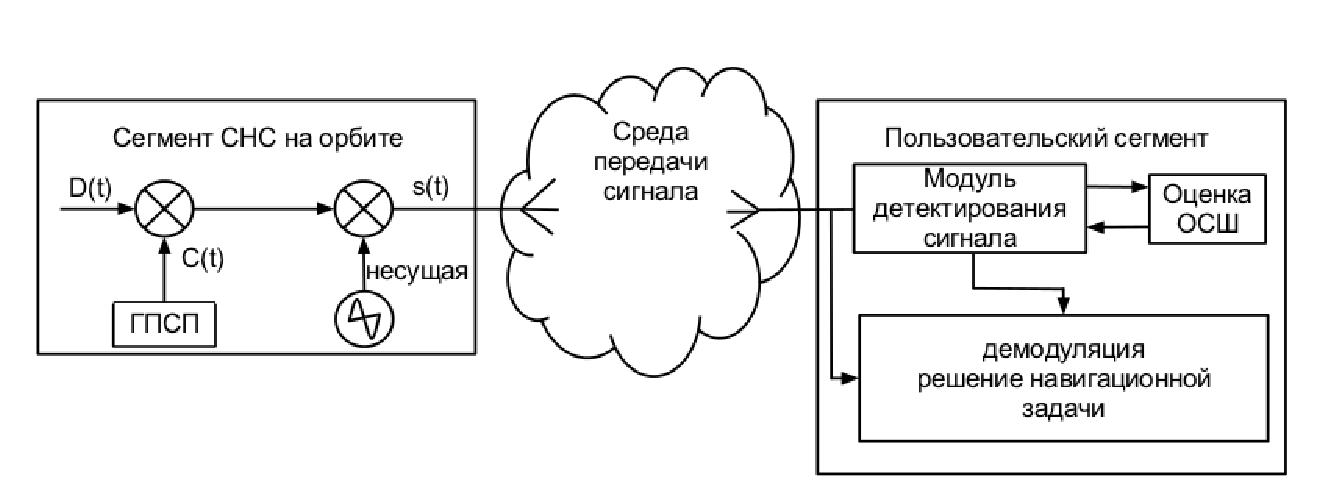
\includegraphics[width=1\linewidth]{sec1gnss_system.eps}}
\caption{структутраная схема СНС GPS}
\label{pic:sec1_gnss_system}
\end{figure}

В систему СНС GPS входят космический сегмент, наземный сегмент (на рисунке \ref{pic:sec1_gnss_system} не
отражен), а так же пользовательский сегмент. В космический сегмент входит спутниковая группировка, в 
наземный - станции управления, в пользовательский - все устройства принимающие сигнал от СНС GPS.

В данной работе рассматривается только пользовательский сегмент. В частности модули детектирования сигнала,
а так же модули оценки ОСШ принятого сигнала. Далее рассмотрены несколько алгоритмов детектирования сигнала,
а так же алгоритмов оценки ОСШ. Но до рассмотрения алгоритмов обработки сигнала, целесообразно кратко 
отразить свойства, а так же методы модулирования сигналов применяемых в СНС GPS.

\subsection{Свойства сигнала СНС GPS}
В системе СНС GPS применяются широкополосные сигналы (ШПС).
ШПС - сигналы, ширина полосы, используемой для передачи сигнала, которых
намного шире минимальной, необходимой для передачи данных \cite{sklyar}. Система связи считается системой с расширенным
спектром в следующих случаях \cite{sklyar}:

\begin{enumerate}
	\item Используемая полоса значительно шире минимальной, необходимой для передачи данных.
	\item Расширение спектра производится с помощью так называемого расширяющего (кодового) сигнала,
		который не зависит от передаваемой информации.
	\item Восстановление исходных данных ("сужение спектра") осуществляется путем сопостовления полученного
		сигнала и синхронизированной копии расширяющего сигнала
\end{enumerate}
Так же подобные сигналы называют:
\textquotedblleftсложными\textquotedblright,
\textquotedblleftшумоподобными\textquotedblright,
\textquotedblleftпсевдослучайными\textquotedblright,
\textquotedblleftсложными-дискретными\textquotedblright,
\textquotedblleftдискретно-кодированными\textquotedblright,
\textquotedblleftортогональными (квазиортогональными)\textquotedblright,
\textquotedblleftоптимальными дискретными\textquotedblright
\cite{gantmaher-book}.
Каждое название ставит акцент на определенной характеристике сигнала. В данной работе я буду оперировать термином
широкополосный сигнал - ШПС. ШПС можно определить как \cite{gantmaher-book, varakin-book}:

\begin{center}
\begin{equation}
	\label{eq:ss_signal}
	1 << FT = B,
\end{equation}
\end{center}
где: ${B}$ - база сигнала, ${F}$ - эффективная ширина спектра, а ${T}$ - длительность.
Неточность этого определеная рассмотрена в \cite{gantmaher-book}, так же там даны ссылки на другие источники
разделяющие критику данного определения. Для данной работы критика, рассмотренная в приведенных источниках,
принципального значения не имеет.

В данной работе используется сигнал с расширенным спектром методом "прямой последовательности". Данный метод
заключается в том, что несущая сигнала модулируется высокоскоростным (широкополосным) расширяющим сигналом \cite{sklyar}.
Методы генерации таких последовательностей рассмотрены, например, в \cite{gantmaher-book}. Это отдельная большая
тема для исследований. В данной работе используется ПСП - код Гоулда. Свойства ПСП подробно рассмотрены в
\cite{gold-ieee}, а так же краткое описание свойств без доказательства приведены в \cite{tsui, akos-book}.

Метод генерирования ПСП подробно рассмотрен во многих источниках \cite{tsui, akos-book, kaplan}
и в данной работе рассматриваться не будет.

В системе СНС GPS применяется двоичная фазовая манипуляция (ДФМ или в иностранной литературе BPSK).
В вышеприведенной системе несущее колебание ${\cos(\omega_{c}t})$ модулируется битами данных ${D_k(t)}$ и битами ПСП
${C_k{t}}$. Принимая во внимание, что потоки битов ${D_k(t)}$ и ${C_k{t}}$ могут принимать значения
${\{+1, -1\}}$. Определим входной сигнал как:

\begin{center}
\begin{equation}
	\label{eq:gps_signal}
	s_k(t) = \sqrt{2A}(C_k(t)D_k(t))\cos(\omega_{c}t)
\end{equation}
\end{center}
где: ${A}$ - мощность сигнала, ${C_k}$ - ПСП для ${k}$ - сигнала, ${D}$ - данные, а ${\omega_{c}t}$ - частота несущей сигнала.

Учитывая, что поток битов может принимать 2 дискретных значения, выражение \ref{eq:gps_signal} можно представить в виде \cite{sklyar}:
\begin{center}
\begin{equation}
	\label{eq:gps_signal_phase}
	s_k(t) = \sqrt{2A}\cos(\omega_{c}t + \phi_{i}(t))
\end{equation}
\end{center}
где: ${A}$ - мощность сигнала, ${\omega_{c}t}$ - частота несущей сигнала, а ${\phi_{i}(t)}$ - фаза несущей сигнала.

Поскольку мы имеем дело с ДФМ, фазовый член выражения \ref{eq:gps_signal_phase} может быть представлен как
${\phi_{i}(t) = \pi_{i}}$. На \ref{pic:sec1_bpsk} представлена несущяя сигнала с ДФМ.

\begin{figure}[ht]
\center\scalebox{0.7}{\includegraphics[width=1\linewidth]{bpsk.eps}}
\caption{Сигнал с модуляцией ДФМ}
\label{pic:sec1_bpsk}
\end{figure}
На рисунке \ref{pic:sec1_bpsk} представлена несущая, модулированная ДФМ.

Демодуляция производится повторной модуляцией принятого сигнала с синхронизированной копией ПСП ${C_k(t) - \tau}$, где
${\tau}$ - оценка фазы ПСП. При идеальной синхронизации сигнала, представленного вырежением \ref{eq:gps_signal},
c локальной копией ПСП, после демодуляции получаем:
\begin{center}
\begin{eqnarray}
	\label{eq:gps_signal_modulated}
	s_k(t) & = & \sqrt{2A}(C^2_k(t)D_k(t))\cos(\omega_{c}t) \\
	& = &\sqrt{2A}D_k(t)\cos(\omega_{c}t)
\end{eqnarray}
\end{center}
Таким образом, на выходе демодулятора получается сигнал с суженным спектром. Следует отметить, что правильная оценка ${\tau}$
является одной из основных задач при детектировании сигнала, так как ПСП имеет пик корреляции только в пределах центрального пика
АКФ \cite{gold-ieee}  - синхронизация с точностью до одного чипа. При неверной оценке фазы ПСП в результате демодуляции спектр
ШПС не будет сужен, что приведет к ошибочным результатам на следующих этапах решения: вычислении уровня шума и принятии решения
о наличии или отсутсивии сигнала заданного спутника в анализируемых данных.

\begin{figure}[H]
\center\scalebox{0.5}{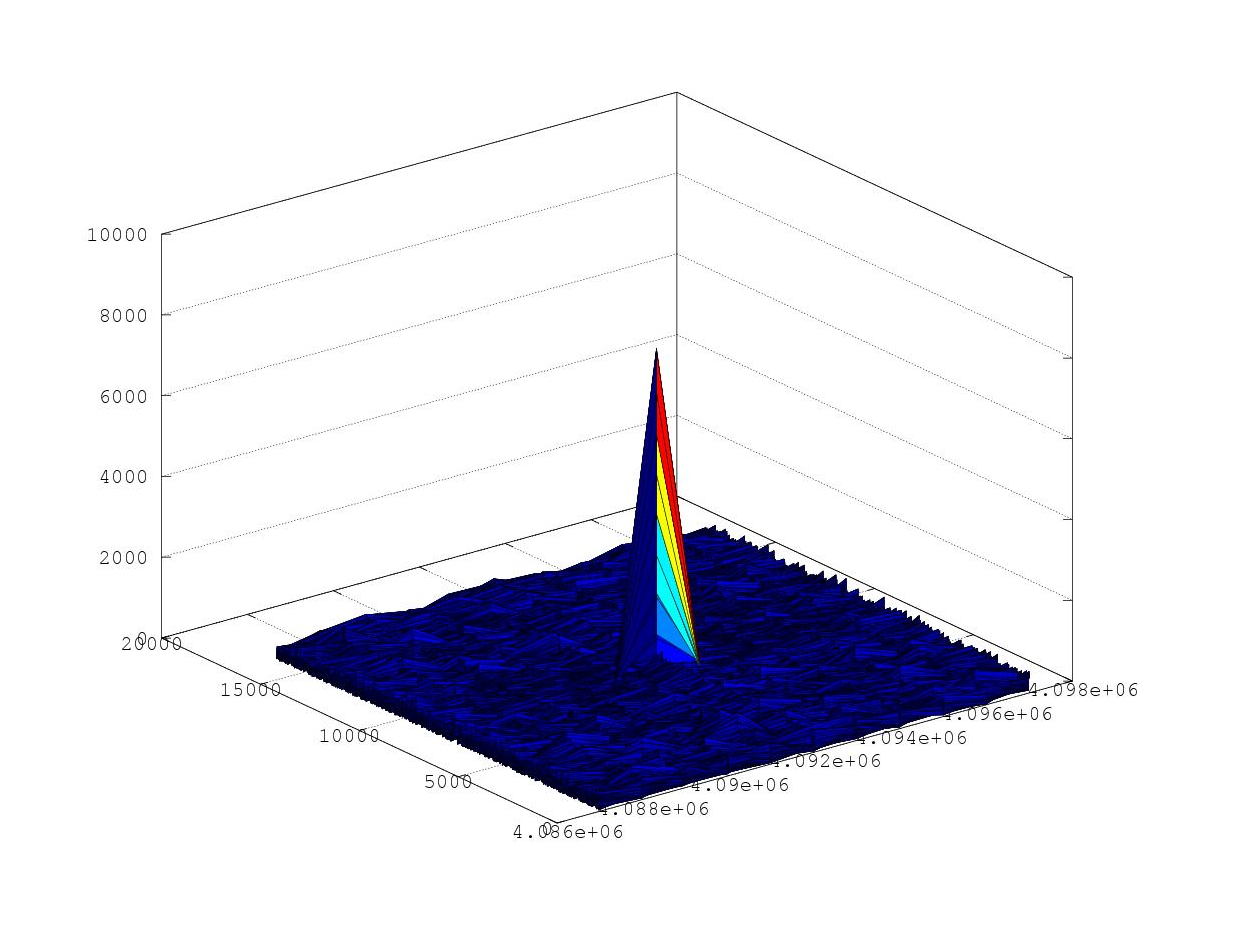
\includegraphics[width=1\linewidth]{corr_peak.eps}}
\caption{График ФН}
\label{pic:corr_peak}
\end{figure}

Задача поиска сигнала сводится к устранению неопределенности по двум параметрам: центральной частоте его спектра
и фазе ПСП. На рисунке \ref{pic:ambiguity_region} представлена область неопределенности. Можно заметить, что сечение
области неопределенности плоскостью ${f}$ представляет собой КФ сигнала. Поиск сигнала соответствует поиску и
оценке основного пика КФ.

\begin{figure}[H]
\center\scalebox{0.5}{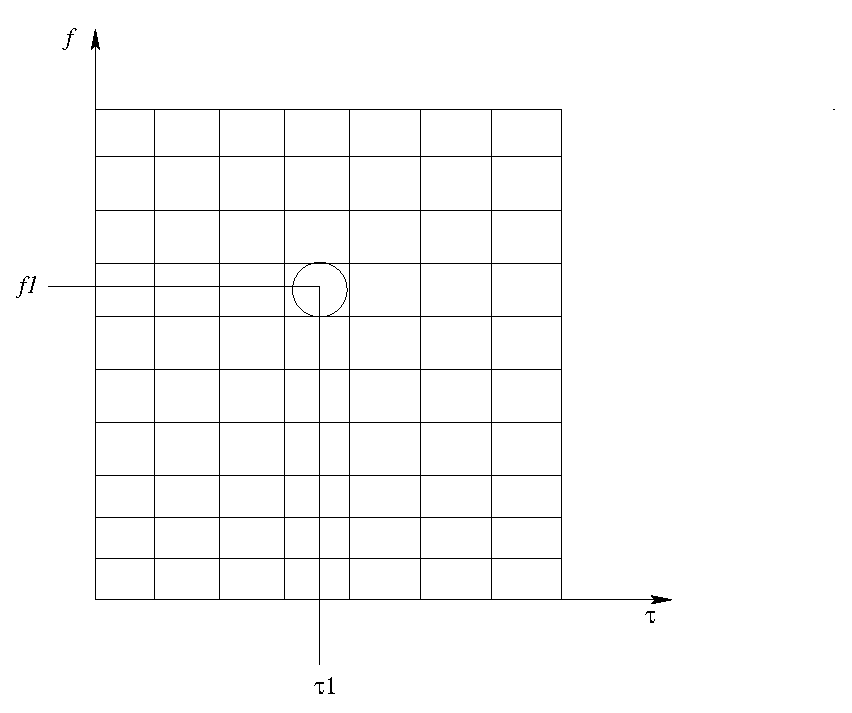
\includegraphics[width=1\linewidth]{ambiguity_region.eps}}
\caption{Область неопределенности}
\label{pic:ambiguity_region}
\end{figure}

\newpage
		% базовая постановка вопроса

% detection 
\subsection{Алгоритм последовательный коррелятор}
\label{sec1_serial}

Данный алгоритм в некоторых источниках так же называется согласованным фильтром. В \cite{sklyar} рассмотрены нюансы этих двух понятий.
В данной работе мы будем использовать понятие последовательный коррелятор. Работа коррелятора описывается математической операцией
корреляции \ref{eq:serial_corr}. Сигнал коррелируется с локальной копией и на выходе коррелятора получается значение, отражающее
степень совпадения сигналов. Не трудно представить, что сигнал с хорошими корреляционными свойствами должен обладать высоким значением
корреляции когда сигналы синхронизированы и минимальным значением в любом другом случае (фаза ПСП-кода не выровнена, отсутствие сигнала).

\begin{equation}
	\label{eq:serial_corr}
	y(n)=\sum\limits_{m=0}^{N-1}{x(m)h(n+m)}
\end{equation}
где: ${x(m)}$ - принятый сигнал, а ${h(n)}$ не импульсная характеристика системы, а локальная копия сигнала.

\newpage
 		%
\subsubsection{Детектирование слабого сигнала с помощью осциллятора Дуффинга}
\label{ssec:duffing}

Детектирование сигналов с расширенным спекторм (в частности сигналов системы Navstar GPS) с помощью осциллятора Дуффинга
достаточно новое направление в исследованиях по данной тематике. В частности
\cite{chaos_chen, chaos_cambridge, chaos_huang, chaos_song}. Так же является интересной более ранняя статья не рассматривающая GPS
\cite{chaos_wang}.

Осциллятор Дуффинга с периодическим внешним воздействием может быть описан уравнением \ref{eq:duffing}:

\begin{center}
\begin{equation}
	\label{eq:duffing}
	mx'' + cx' + k_{1}x + k_{2}x^3 = F_{0}\cos(\omega{t})
\end{equation}
\end{center}

где
$m$- масса,
$c$ - коэффициент диссипации,
$x$ - состояние осциллятора,
$k_1$ и $k_2$ - линейный и нелинейный коэффициенты соответственно.
$F_{0}\cos(\omega{t})$ - внешнее воздействие.

Подробно уравнение \ref{eq:duffing} рассмотрено в \cite{chaos_neimark_landa} (Глава 9 параграф 3). Но
для использования осциллятора Дуффинга для детектирования сигналов системы GPS былa предложена
усовершенствованная форма данного осциллятора \cite{chaos_song, chaos_chen}:

\begin{center}
\begin{equation}
	\label{eq:duffing_gps}
	x'' +cx' - x^3 + x^5 = \gamma\cos(\omega{t}) + (\gamma_{x}\cos(\omega_{x}) + n(t))
\end{equation}
\end{center}

Перепишем динамическую систему \ref{eq:duffing_gps} в виде:
\begin{center}
\begin{eqnarray}
	\label{eq:duffing_gps_2}
	y(t) & = & x'(t) \\
	y'(t) & = & -cx' + x^3 - x^5 + \gamma\cos(\omega{t}) + (\gamma_{x}\cos(\omega_{x}) + n(t))
\end{eqnarray}
\end{center}

Пример фазового портрета при ${\omega=\omega_{x}}$ изображен на рисунке \ref{pic:duffing_sync},
фазовый портрет хаоса расположен на рисунках \ref{pic:duffing_chaos1}, \ref{pic:duffing_chaos2}

\begin{figure}[H]
	\center\scalebox{0.5}{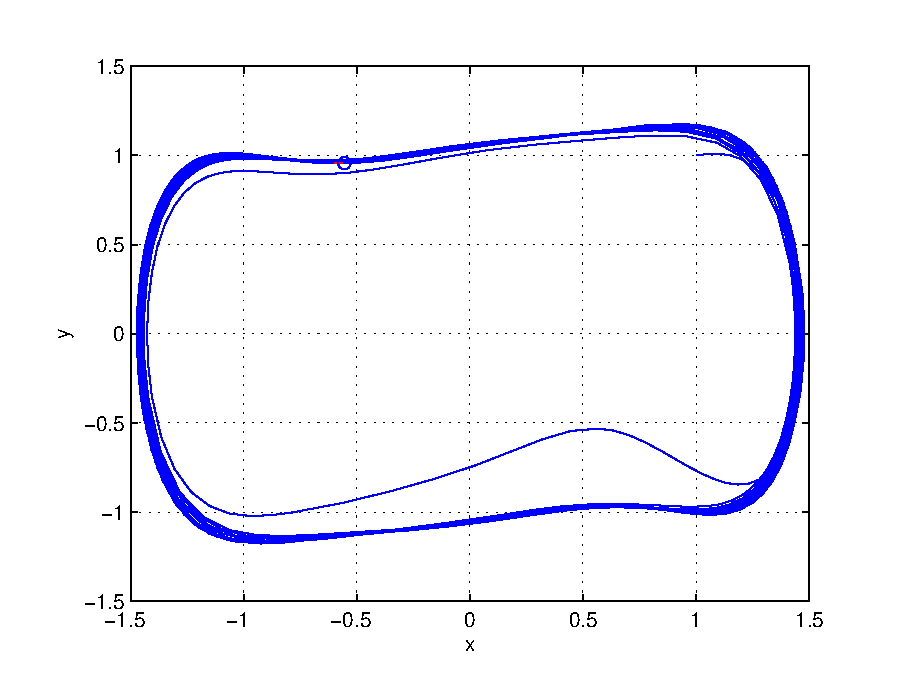
\includegraphics[width=1\linewidth]{duffing_sync.eps}}
	\caption{Фазовый портрет при ${\omega =\omega_{x}}$}
	\label{pic:duffing_sync}
\end{figure}

\begin{figure}[H]
	\center\scalebox{0.5}{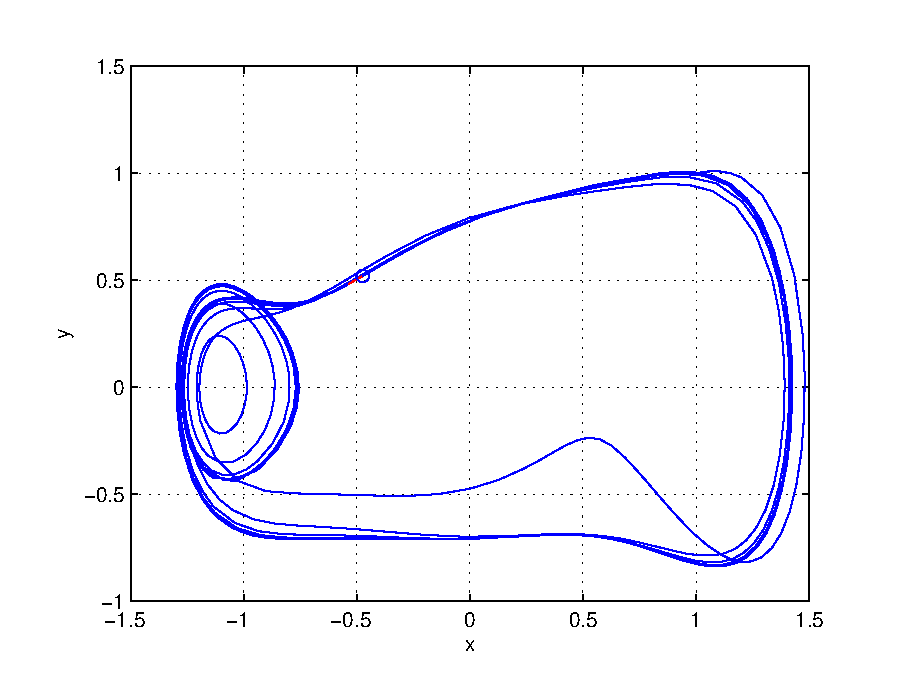
\includegraphics[width=1\linewidth]{duffing_chaos1.eps}}
	\caption{Фазовый портрет при ${\omega < \omega_{x}}$}
	\label{pic:duffing_chaos1}
\end{figure}

\begin{figure}[H]
	\center\scalebox{0.5}{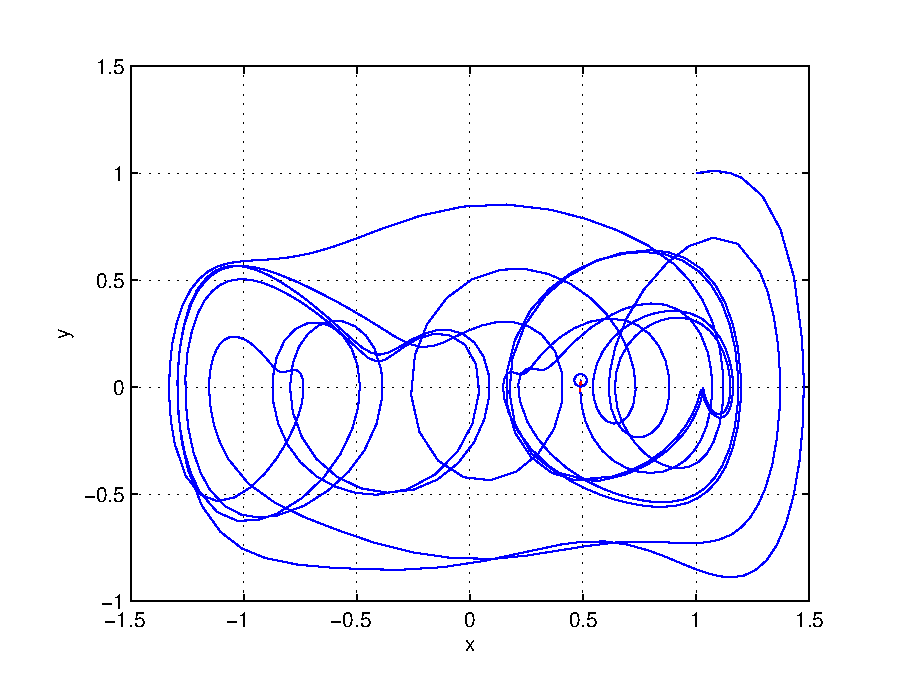
\includegraphics[width=1\linewidth]{duffing_chaos2.eps}}
	\caption{Фазовый портрет при ${\omega > \omega_{x}}$}
	\label{pic:duffing_chaos2}
\end{figure}

В качестве параметров уравнения применялись $c = 0.5$, $\gamma=\gamma_{x}=0.36$, ${\omega=1}$

Часто для вычисления характеристик хаотической динамики применяется экспонента Ляпунова.
Она описывает метод определения в каком состоянии находится система. Если система находится
в стабильном состоянии линии фазовой траектории будут близко прилегать одна к другой, в противном
случае система находится в состоянии хаоса.

В статье \cite{chaos_chen} предложен усовершенствованный метод, базирующийся на вычислении дисперсии
фазовой траектории. Действительно, на рисунках \ref{pic:duffing_sync}, \ref{pic:duffing_chaos1},
\ref{pic:duffing_chaos2} видно - когда система находится в хаотическом состоянии значение
дисперсии по координате ${x}$, чем соответствующее значение в состоянии $\omega = \omega_{x}$.
На основе этого была предложена усовершенствованная схема детектора сигнала
\ref{pic:chaos_energy_detector}

\begin{figure}[H]
	\center\scalebox{0.7}{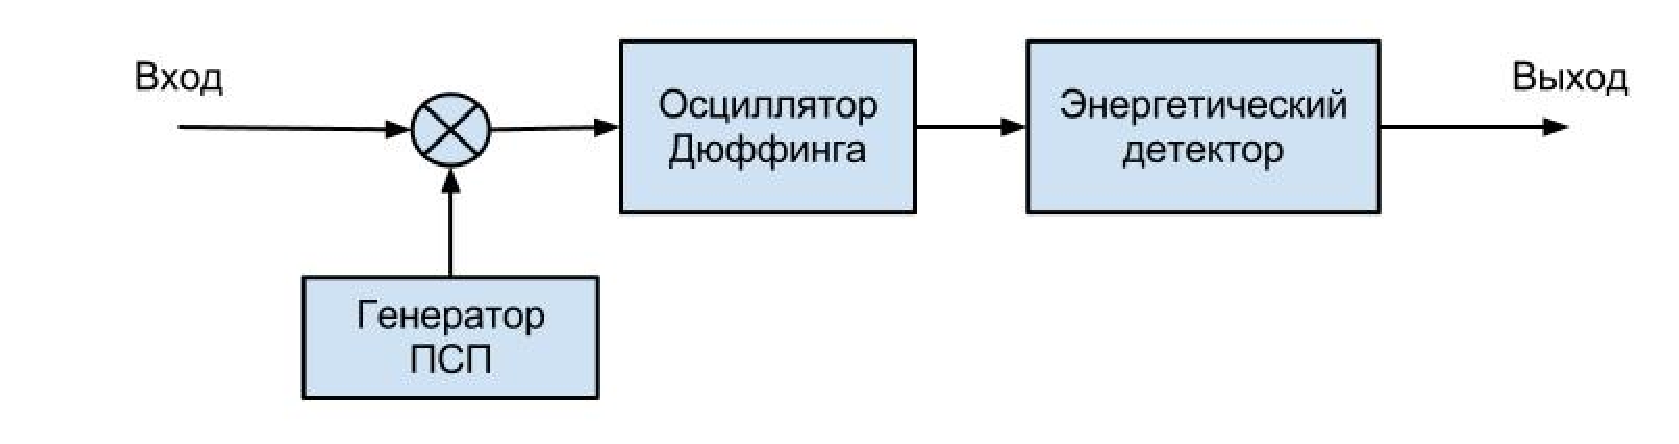
\includegraphics[width=1\linewidth]{chaos_detector.eps}}
	\caption{Схема энергетического детектора для осциллятора Дуффинга}
	\label{pic:chaos_energy_detector}
\end{figure}

\newpage
		%
\subsection{Алгоритм детектирования с применением статистик высоких порядков}
\label{sbs:sec1_hos}

Математический аппарат статистик высоких порядков (СВП или HOS - Higher-order statistics)
для исследования не причнинных, причинных и нестабильных
(систем с не минимальной фазой) и не-Гауссовых сигналов впервые был предложен в \cite{hos_petropulu} в 1993 году.
Этот метод позволяет не только подавлять цветной Гауссов шум, но так же в некоторых случаях подавлять
цветной не-Гауссов шум.

В работе \cite{hos_zhao} был предложен метод детектирвоания ШПС с использованием СВП.

\newpage
		% Higher-order statistics

%optimization
\subsection{Метода оптимизации алгоритмов}
\subsubsection{Коррелятор}

\paragraph{Параллельный коррелятор}
\label{sec1_fft}
Вычисление циклической свертки через дискретное преобразование Фурье (ДПФ) является достаточно популярным методом
в программных приемниках, так как позволяет существенно 
уменьшить количество элементарных операций при вычислении. Но как показано в \cite{tsui, oppenheim} можно достаточно просто
перейти от свертки к циклической корреляции. Так как этот метод является самым популярным в программных приемниках, рассмотрим его
подробнее.

Обозначим импульсный отклик системы через $h(n)$, а через ${x(n)}$ - входной сигнал. Тогда выходной сигнал в дискретном
временной домене можно записать как:

\begin{equation}
	\label{eq:fft_conv}
	y(n)=\sum\limits_{m=0}^{N-1}{x(m)h(n-m)}
\end{equation}

Стоит отметить, что в \ref{eq:fft_conv} сдвиг во времени является циклическим, поскольку дискретные операции являются циклическими.
Возьмем ДПФ от \ref{eq:fft_conv}

\begin{center}
\begin{eqnarray}
	\label{eq:fft_conv_fft}
	Y(k) & = & \sum\limits_{n=0}^{N-1}\sum\limits_{m=0}^{N-1}{x(m)h(n-m)e^{(-j2\pi{kn})/N}}=\nonumber \\
	& = & \sum\limits_{m=0}^{N-1}{x(m)}[\sum\limits_{n=0}^{N-1}h(n-m)e^{(-j2\pi{(n-m)}k)/N}]e^{(-j2\pi{m}k)/N}=\\
	& = & H(k)\sum\limits_{m=0}^{N-1}e^{(-j2\pi{m}k)/N} = X(k)H(k)\nonumber 
\end{eqnarray}
\end{center}


Из уравнения \ref{eq:fft_conv_fft} легко видеть, что это не линейная свертка. В линейной свертке для $N$ входного
сигнала и свертки результатом будет $2N-1$ точек. А в уравнении выше, результатом является всего $N$ точек.
Это является результатом циклической природы ДПФ.

Алгоритм детектирования не использует свертку, он использует корреляцию, которая отличается от свертки. Корреляция
между $x(n)$ и $h(n)$ может быть записана как:

\begin{equation}
	\label{eq:fft_corr}
	y(n) = \sum\limits_{m=0}^{N-1}{x(m)h(n+m)}
\end{equation}
Единственным отличаем между \ref{eq:fft_conv} и \ref{eq:fft_corr} является знак перед $m$ в ${h(n+m)}$.
В случае детектирования сигнала $h(n)$ является локальной копией сигнала, а не импульсной характеристикой.
Произведем ДПФ над $z(n)$:

\begin{center}
\begin{eqnarray}
	\label{eq:fft_corr_fft}
	Z(k) & = & \sum\limits_{n=0}^{N-1}\sum\limits_{m=0}^{N-1}{x(m)h(n+m)e^{(-j2\pi{kn})/N}}=\nonumber \\
	& = & \sum\limits_{m=0}^{N-1}{x(m)}[\sum\limits_{n=0}^{N-1}h(n+m)e^{(-j2\pi{(n+m)}k)/N}]e^{(j2\pi{m}k)/N}=\\
	& = & H(k)\sum\limits_{m=0}^{N-1}e^{(j2\pi{m}k)/N} = X(k)H^{-1}(k)\nonumber 
\end{eqnarray}
\end{center}
где ${X^{-1}(k)}$ - обратное ДПФ. Уравнение \ref{eq:fft_corr_fft} можно записать как:

\begin{equation}
	\label{eq:fft_corr_fft_rev}
	Y(k) = \sum\limits_{n=0}^{N-1}\sum\limits_{m=0}^{N-1}{x(n+m)h(m)e^{(-j2\pi{kn})/N}}=X^{-1}(k)H(k)
\end{equation}

Если сигнал $x(n)$ реальный, то $x(n) = x^*(n)$, где * - операция комплексного сопряжения. Используя данное соотнешение,
значение $Z(k)$ может быть записано:
\begin{equation}
	\label{eq:fft_magnitude}
	|Z(k)|=|H^*(k)X(k)|=|H(k)X(k)^*|
\end{equation}
Данное соотношение может быть использовано для нахождения значения циклической корреляции между входным сигналом и 
локальной копией.



\newpage
	%
\subsection{Алгоритм delay and multiply approach}
\label{ssec:dma}

Алгоритм был предаставлен в книге и статье американского ученого Дж.
Цуя \cite{lin_dma, tsui}

Пусть входной комплексный сигнал описывается формулой \ref{eq:dma_lo_signal}:

\begin{center}
\begin{equation}
	\label{eq:dma_lo_signal}
	s(t)=A(t)e^{j2{\pi}f_{0}t}
\end{equation}
\end{center}

где $A(t)$ - амплитуда, а $f_{0}$- частота несущей сигнала.

Если входящий комплексный сигнал имеет задержку $\tau$, то данный
сигнал будет описываться формулой: 

\begin{center}
\begin{equation}
	\label{eq:dma_signal}
	s(t-\tau)=A(t-\tau)e^{j2{\pi}f_{0}(t-\tau)}
\end{equation}
\end{center}

Получим новый сигнал путем умножения \ref{eq:dma_lo_signal} и \ref{eq:dma_signal}:

\begin{center}
\begin{eqnarray}
	s_{n}(t) & = & s(t)s(t-\tau)^{*}=\nonumber \\
	 & = & A(t)A(t-\tau)e^{j2\pi f_{0}t}e^{j2\pi f(t-\tau)}=\label{eq:dma}\\
	 & = & A(t)A(t-\tau)e^{j2\pi f_{0}\tau}\nonumber 
\end{eqnarray}

\par\end{center}

Из формулы \ref{eq:dma} видно, что полученный сигнал не зависит от
задержки $\tau$. Остается найти фазу C/A кода. Референсный сигнал
$A(t)A(t-\tau)$ используется для корреляции с новым кодом, который
получен по формуле \ref{eq:dma} - умножением принятого сигнала и его задержанной
копии. Когда фаза C/A кода найдена, поиск сводится к одномерному поиску
частоты. Данный метод позволяет уменьшить количество вычислений, путем
сведения задачи поиска в двух измерения: по фазе кода и частоте; к
задаче поиска только по частоте. Этот метод позволяет существенно
сэкономить вычислительные ресурсы при обнаружении сигнала заданного
спутника, но, вместе с тем, операция умножения повышает шум в процессе.

\subsubsection{Aнализ изменения ОСШ при использовании алгоритма DMA}
\label{sssec:dma_noise}

Воспользуемся математическим аппаратом теории вероятностей. Необходимый математический аппарат
рассотрен в \cite{ventcel}, для более подробного изучения можно ознакомиться с \cite{feller}.

Добавим в формулу \ref{eq:dma} АБГШ:

\begin{center}
\begin{eqnarray}
	s_{n}(t) & = & (s(t)+n_{1}(t))(s(t-\tau)+n_{2}(t))^{*}=\nonumber \\
	 & = & A(t)A(t-\tau)e^{j2{\pi}f_{0}{\tau}}+\nonumber \\
	 & + & A(t)e^{j2{\pi}f_{0}t}n_{2}(t)+\label{eq:dma_noise}\\
	 & + & A(t-\tau)e^{j2{\pi}f_{0}(t-\tau)}n_{1}(t)+\nonumber \\
	 & + & n(t)^{2}\nonumber 
\end{eqnarray}
\end{center}

где
$A(t)A(t-\tau)e^{j2{\pi}f_{0}{\tau}}$ - новая ПСП, а
$A(t)e^{j2{\pi}f_{0}t}n_{2}(t)+A(t-\tau)e^{j2{\pi}f_{0}(t-\tau)}n_{1}(t) + n(t)^{2}$ -
шумовая компонента.

Свойства дисперсии случайных величин рассмотрены в \cite{ventcel}. Дисперсия суммы 
независимых случайных величин приведена на формуле \ref{eq:var_add_full}:

\begin{center}
\begin{equation}
	\label{eq:var_add_full}
	D[\sum\limits_{i=1}^{n}{X_i}]=\sum\limits_{i=1}^{n}{D[X_i]} + 2\sum\limits_{i<j}{K_{ij}}
\end{equation}
\end{center}

Для некореллированных случайных величин можно формулу \ref{eq:var_add_full} переписать как \ref{eq:var_add}:

\begin{center}
\begin{equation}
	\label{eq:var_add}
	D[\sum\limits_{i=1}^{n}{X_i}]=\sum\limits_{i=1}^{n}{D[X_i]}
\end{equation}
\end{center}

Дисперсия произведения независимых случайных величин может быть представлена как \ref{eq:var_mult}:
\begin{center}
\begin{equation}
	\label{eq:var_mult}
	D[\prod\limits_{i=1}^{n}{X_i}]=\prod\limits_{i=1}^{n}{(D_i + m_{i}^{2})} - \prod\limits_{i=1}^{n}{m_{i}^{2}}
\end{equation}
\end{center}

Вернемся к рассмотрению формулы \ref{eq:dma_noise}.

\subsubsection{Результаты моделирования}
\label{sssec:dma_simulate}

\newpage
		%
\subsection{Алгоритм нахождения пика AКФ}

Данный алгоритм представлен в работах \cite{2max_ieee, 2max_article}. Его оригинальное название
\textquotedblleft{Peak-finding algorithm}\textquotedblright,
в данной работе введем перевод -
\textquotedblleft{Алгоритм нахождения пика}\textquotedblright (АНП). 

Алгоритм был разработан для улучшения рабочих характеристик традиционных алгоритмов рассмотренных в
\ref{sec1_serial} и \ref{sec1_fft}. Предложенный алгоритм можно разбить на несколько шагов:
\begin{itemize}
\item[Шаг 1] Подсчитать АКФ, используя метод предложенный в \ref{sec1_fft}.
\item[Шаг 2] Найти главный пик АКФ, найти второй пик АКФ, найти среднее значение АКФ.
\item[Шаг 3] Нормализовать полученные значения относительно главного пика АКФ.
\item[Шаг 4] Если (максимум АКФ - среднее) > ${V_{th1}}$ и (максимум АКФ - 
	второй максимум АКФ) > ${V_{th2}}$, тогда полученный главный пик АКФ соответсвует
	искомой фазе кода и частоте.
\end{itemize}

В статье авторов \cite{2max_ieee} предложенны следующие значения для порогов:
${V_{th1}} = 0.3$(Дб) и  ${V_{th2}} = 0.15$(Дб). Так же авторы предлагают итерационную процедуру для нахождения
фазы ПСП и частоты смещения допплера:
\begin{itemize}
\item[Шаг 1] Начать вычисление с 1мс.
\item[Шаг 2] Получить результаты АНП.
\item[Шаг 3] Если фаза ПСП и частота не могут быть найдены, увеличить время интегрироавния сигнала.
	Использовать следующие значения для интегрирования: 1мс -> 10мс -> 50мс -> 100мс -> 200мс ->
	500мс -> 1000мс
\end{itemize}

%\begin{center}
%\begin{equation}
%	\label{eq:dma_signal}
%	SNR(dB) = 10\log{\frac{max[d(n)] - mean[d(n)]}{std[d(n)]}}
%\end{equation}
%\end{center}

\newpage
		%

% noise
\subsection{Постановка задачи оценки шума}
\label{sssec:sec1_noise_est}

Задача оценки отношения сигнал-шума (ОСШ) является одной из ключевых при детектировании сигналов.
ОСШ используется в задаче определения порога детектирования рисунок \ref{pic:sec1_gnss_system}.
При превышении порога принимается решение о наличии сигнала в принимаемой смеси, если же порог
не превышен, считается, что сигнал данного в смеси не присутствует.

Пусть для данной задачи входной сигнал описывается соотношением \cite{presti_ieee}:
\begin{center}
\begin{equation}
	\label{eq:noise_est_signal}
	s_C[n]=\sqrt{P_d}D[n] + \sqrt{P_n}\eta[n]
\end{equation}
\end{center}
где $D[n]$ - биты навигационного сообщения, $\eta[n]=\eta_{Re} + j\eta_{Im}$ - комплексный шум,
$P_d$ - мощность сигнала, а $P_n$ - мощность шума (обе величины берутся на выходе коррелятора).
Стоит отметить, что $D[n]=b_{n}e^{j\theta_n}$, где $b_n=\pm{1}$ для сигналов с двоичной модуляцией, а
$\theta_n$ - остаточная фазовая ошибка от контура ФАПЧ слежения за частотой.
Тогда ОСШ для $s_C[t]$ можно представить как:
\begin{center}
\begin{equation}
	\label{eq:noise_est_snr}
	R_e=\frac{P_d}{P_n}
\end{equation}
\end{center}
%От выражения \ref{eq:noise_est_snr} можно перейти к соотношению количества шума на герц $C/N_0$:
%\begin{center}
%\begin{equation}
%	\label{eq:noise_est_cn}
%	R_e=\frac{C}{N_{0}B_{eqn}}\Rightarrow\frac{C}{N_0}=R_e B_{eqn}
%\end{equation}
%\end{center}
%где ${B_{eqn}}$ - нормализованная эквивалентная шумовая полоса
%В \cite{presti_ieee} показано, что $B_{eqn}$ можно выразить:
%\begin{center}
%\begin{equation}
%	\label{eq:noise_est_beqn}
%	B_{eqn}=\frac{1}{T_{int}}
%\end{equation}
%\end{center}
%где ${T_{int}}$ - время интегрирования.

%%%%%%%%%%%%%%%%%%%%%%%%%%%%%%%%%%%%%%%%%%%%%%%%%%%%%%
\subsubsection{Алгоритм оценки ОСШ
\textquotedblleftдействительный сигнал - комплексный шум\textquotedblright}
\label{sssec:rscn}
В иностранной литературе он называется "Real Signal - Complex Noise (RSCN)". Введем перевод
"Действительный сигнал - комлексный шум (ДСКШ)".
Данный алгоритм рассмотрен в статьях \cite{badke_rscn, presti_insidegnss, presti_ieee}.

Если рассматривать идеально синхронизированный сигнал, тогда в синфазном контуре будет
находится сигнал и АБГШ, в то время как в квадратурном плече будет находится только шум,
независимый и одинаково распределенный с шумом в синфазном контуре. Данный факт может
быть использован для оценки ОСШ в программном приемнике:
\begin{center}
\begin{equation}
	\label{eq:rscn_noise_power}
	\hat{P_n} = \frac{2}{N}\sum^N_{v=1}|s_{C,Im}[v]|^2
\end{equation}
\end{center}
где ${s_{C,Im}[v]}$ - мнимая часть от ${s_C}$.

\begin{center}
\begin{equation}
	\label{eq:rscn_total_power}
	\hat{P}_{tot} = \frac{1}{N}\sum^N_{v=1}|s_{C}[v]|^2
\end{equation}
\end{center}
где ${P_{tot}}$ - оценка энергии смеси.

\begin{center}
\begin{equation}
	\label{eq:rscn_data_power}
	\hat{P_d} = \hat{P}_{tot} - \hat{P_n}
\end{equation}
\end{center}

\begin{center}
\begin{equation}
	\label{eq:rscn_snr}
	\hat{R_e} = \frac{\hat{P_d}}{\hat{P_n}} = \frac{\hat{P}_{tot} - \hat{P_n}}{\hat{P_n}} 
\end{equation}
\end{center}

Очевидно, что данный метод является чувствительным к сдвигу фазы, который приводит к переходу энергии
в квадратурный контур. Любой остаточный сдвиг фазы ведет к возрастанию энергии шума в квадратурном
контуре (это видно из \ref{eq:rscn_noise_power}).

%%%%%%%%%%%%%%%%%%%%%%%%%%%%%%%%%%%%%%%%%%%%%%%%%%%%%%
\subsubsection{Алгоритм Signal-to-Noise Variance}
\label{sssec:snv}

Данный алгоритм был представлен в \cite{snr_pauluzzi, snr_li}. Квадратичный ОСШ оценщик, основан на 1
и 2 моменте семплов сигнала:

\begin{center}
\begin{equation}
	%\label{eq:rscn_data_power}
	\hat{P_{d}} = (\frac{1}{N} \sum \limits_{v=1}^N \left| s_{C,Re}[v] \right|)^2
\end{equation}
\end{center}
где ${s_{C,Re}[v]}$ - действительная часть от ${s_C}$.

\begin{center}
\begin{equation}
	%\label{eq:rscn_data_power}
	\hat P_{tot} = \frac{1}{N} \sum \limits_{v=1}^{N} \left|s_C[v] \right| ^2
\end{equation}
\end{center}

\begin{center}
\begin{equation}
	%\label{eq:rscn_snr}
	\hat{R_e} = \frac{\hat P_d}{\hat P_{tot} - \hat P_d}
\end{equation}
\end{center}

%%%%%%%%%%%%%%%%%%%%%%%%%%%%%%%%%%%%%%%%%%%%%%%%%%%%%%
\subsubsection{Алгоритм Beaulieu}
\label{sssec:beaulieu}

Данный алгоритм был представлен в статье \cite{snr_beaulieu}.
\begin{center}
\begin{equation}
	%\label{eq:rscn_data_power}
	\hat{P_{n,v}} = (\left| r_{C,Re}[v] \right| - \left| r_{C,Re}[v-1] \right|)^2
\end{equation}
\end{center}
где случайная величина ${P_{n,v}}$ - мгновенное значение энергии шумовой компоненты ${\eta[v]}$.

\begin{center}
\begin{equation}
	%\label{eq:rscn_data_power}
	\hat{P_{d,v}} = \frac{1}{2}(r_{C,Re}[v]^2 + r_{C,Re}[v-1]^2)
\end{equation}
\end{center}
где случайная величина ${P_{d,v}}$ - мгновенное значение энергии сигнала ${s_C[v]}$.

\begin{center}
\begin{equation}
	%\label{eq:rscn_snr}
	\hat{R_e} = \left[ \frac{1}{N} \sum \limits_{v=1}^{N} \frac{\hat P_{n,v}}{\hat P_{d,v}} \right]^{-1}
\end{equation}
\end{center}

%%%%%%%%%%%%%%%%%%%%%%%%%%%%%%%%%%%%%%%%%%%%%%%%%%%%%%
\subsubsection{Алгоритм основанный на методе моментов}
\label{sssec:mm}
Данный алгоритм был представлен в \cite{snr_pauluzzi}. Он использует 2 и 4 статистические моменты для раздельной оценки
мощности сигнала и шума.
\begin{center}
\begin{equation}
	%\label{eq:rscn_data_power}
	\hat M_2 = \frac{1}{N} \sum \limits_{v=1}^{N} \left|s_C[v] \right| ^2
\end{equation}
\end{center}
\begin{center}
\begin{equation}
	%\label{eq:rscn_data_power}
	\hat M_4 = \frac{1}{N} \sum \limits_{v=1}^{N} \left|s_C[v] \right| ^4
\end{equation}
\end{center}
где ${M_2}$ и ${M_4}$ - 2 и 4 моменты случайной величины.

\begin{center}
\begin{equation}
	%\label{eq:rscn_data_power}
	\hat P_d(M_2, M_4) = \sqrt{2 \hat M^2_2 - \hat M_4} 
\end{equation}
\end{center}

\begin{center}
\begin{equation}
	%\label{eq:rscn_data_power}
	\hat P_n(M_2, M_4) = \hat M_2 - \hat P_d
\end{equation}
\end{center}

\begin{center}
\begin{equation}
	%\label{eq:rscn_snr}
	\hat{R_e} = \frac{\hat{P_d}(\hat{M_2}, \hat{M_4})}{\hat P_n(\hat{M_2}, \hat{M_4})}
\end{equation}
\end{center}

%%%%%%%%%%%%%%%%%%%%%%%%%%%%%%%%%%%%%%%%%%%%%%%%%%%%%%
%\subsubsection{Алгоритм Narrowband-Wideband Power Ratio}
%\label{sssec:nwpr}
%
%Данный алгоритм был представлен в \cite{parkinson_1996}, а так же в нескольких других книгах по СНРС GPS. Особенностью данного алгоритма
%является то, что это единственный алгоритм производящий оценку ${C/N_0}$, а не ОСШ, который может быть преобразован ${C/N_0}$.
%
%\begin{center}
%\begin{equation}
%	%\label{eq:rscn_data_power}
%	WBP_k = \sum \limits_{m=1}^{M} \left|s_C[kM+m] \right| ^2, k=0,1,...(\frac{N}{M}-1)
%\end{equation}
%\end{center}
%
%\begin{center}
%\begin{equation}
%	%\label{eq:rscn_data_power}
%	NBP_k = \left(\sum \limits_{m=1}^{M} \left|s_{C,Re}[kM+m] \right| \right)^2 + \left(\sum \limits_{m=1}^{M} \left|r_{C,Im}[kM+m] \right| \right)^2
%\end{equation}
%\end{center}
%
%\begin{center}
%\begin{equation}
%	%\label{eq:rscn_data_power}
%	\hat \mu_{NP} = \frac{M}{N} \sum \limits_{k=0}^{N/M-1} \frac{NBP_k}{WBP_k}
%\end{equation}
%\end{center}
%
%\begin{center}
%\begin{equation}
%	%\label{eq:rscn_data_power}
%	\gamma = \frac{C}{N_0} = \frac{1}{T_{int}} \frac{\hat \mu_{NP} - 1}{M - \hat \mu_{NP}}
%\end{equation}
%\end{center}

%%%%%%%%%%%%%%%%%%%%%%%%%%%%%%%%%%%%%%%%%%%%%%%%%%%%%%
\subsubsection{Выводы}
Приведенные алгоритмы подробно рассмотрены в \cite{presti_ieee}. Получены их оценки по количеству операций, а так же
исследованы свойства аппроксимации данных функций. Следует отметить, что данные алгоритмы работают только с синхронизированным сигналом.
В виду этого является очень важным получить достаточно точную оценку частоты на ранних стадиях детектирования сигнала

\newpage
		% постановка вопроса оценки шума
% так зверски сделаны кавычки
\subsection{Алгоритм оценки ОСШ
\textquotedblleftдействительный сигнал - комплексный шум\textquotedblright}

В иностранной литературе он называется "Real Signal - Complex Noise (RSCN)". Введем перевод
"Действительный сигнал - комлексный шум (ДСКШ)".
Данный алгоритм рассмотрен в статьях \cite{badke_rscn, presti_insidegnss, presti_ieee}.

Если рассматривать идеально синхронизированный сигнал, тогда в синфазном контуре будет
находится сигнал и АБГШ, в то время как в квадратурном плече будет находится только шум,
независимый и одинаково распределенный с шумом в синфазном контуре. Данный факт может
быть использован для оценки ОСШ в программном приемнике:
\begin{center}
\begin{equation}
	\label{eq:rscn_noise_power}
	\hat{P_n} = \frac{2}{N}\sum^N_{v=1}|r_{C,Im}[v]|^2
\end{equation}
\end{center}

\begin{center}
\begin{equation}
	\label{eq:rscn_total_power}
	\hat{P}_{tot} = \frac{1}{N}\sum^N_{v=1}|r_{C}[v]|^2
\end{equation}
\end{center}

\begin{center}
\begin{equation}
	\label{eq:rscn_data_power}
	\hat{P_d} = \hat{P}_{tot} - \hat{P_n}
\end{equation}
\end{center}

\begin{center}
\begin{equation}
	\label{eq:rscn_snr}
	\hat{\lambda_C} = \frac{\hat{P_d}}{\hat{P_n}} = \frac{\hat{P}_{tot} - \hat{P_n}}{\hat{P_n}} 
\end{equation}
\end{center}

Очевидно, что данный метод является чувствительным к сдвигу фазы, который приводит к переходу энергии
в квадратурный контур. Любой остаточный сдвиг фазы ведет к возрастанию энергии шума в квадратурном
контуре (это видно из \ref{eq:rscn_noise_power}).

\newpage
		% rscn - алгоритм

%Литература
\clearpage
\phantomsection
\addcontentsline{toc}{chapter}{\bibname}	% Добавляем список литературы в оглавление
\bibliography{bibtex_db}
 %
\end{document}
